\chapter{BRINCANDO COM LETRAS E SONS}
\markboth{Módulo 1}{}

\colorsec{Habilidade do SAEB}

\begin{itemize}
\item Relacionar elementos sonoros das palavras com sua representação.
\end{itemize}

\colorsec{Habilidades da BNCC}

\begin{itemize}
\item EF01LP04, EF01LP05, EF01LP07, EF01LP08, EF01LP09.
\end{itemize}

%\coment{Faça uma breve revisão das letras do alfabeto e aponte as relações entre letras e fonemas. Pergunte aos alunos: qual é o som dessa letra? Essa mesma letra representa apenas um som? Que outros sons essa mesma letra pode representar? Depois, de forma lúdica, apresente as vogais, mostrando que elas podem ser todas ditas em sequência; proceda da mesma forma com as consoantes, explicitando que, para construir o som delas, é preciso interromper a passagem do ar em algum momento. Compare sons parecidos. Finalmente, explique as sílabas. }


\conteudo{VOCÊ CONHECE AS LETRAS DO ALFABETO?

AS LETRAS SÃO SINAIS GRÁFICOS USADOS PARA ESCREVER AS PALAVRAS. JUNTAS,
AS 26 LETRAS FORMAM O NOSSO ALFABETO. VEJA:

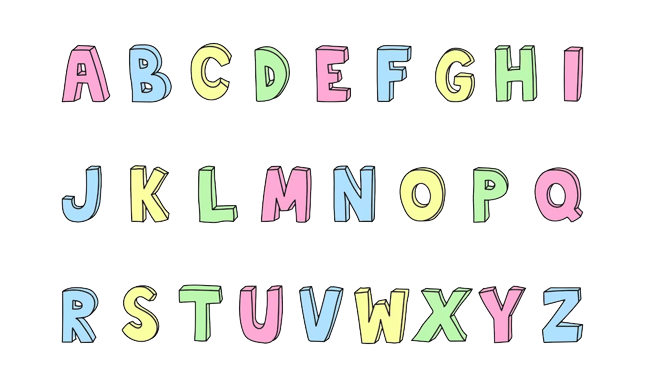
\includegraphics[width=\textwidth]{media/image1.png}

CADA LETRA DO ALFABETO REPRESENTA UM SOM CHAMADO DE FONEMA. SÃO OS FONEMAS QUE DÃO ORIGEM ÀS PALAVRAS. A LETRA H É A ÚNICA LETRA DO ALFABETO QUE NÃO
APRESENTA SOM.}

\conteudo{
O ALFABETO ESTÁ DIVIDIDO EM DUAS PARTE: VOGAIS E CONSOANTES.

AS VOGAIS SÃO A - E - I - O - U, E AS CONSOANTES SÃO B, C, D, F, G, H, J,
L, M, N, P, Q, R, S, T, V, X, Z. AINDA EXISTEM TRÊS CONSOANTES ESPECIAIS - K,
Y, W - QUE SÃO USADAS PARA ESCREVER PALAVRAS DE ORIGEM ESTRANGEIRA.

UMA PALAVRA PODE SER DIVIDIDA EM UM OU MAIS PEDACINHOS CHAMADOS DE
SÍLABAS. AS SÍLABAS DAS PALAVRAS PODEM SER CLASSIFICADAS COMO INICIAIS, MEDIAIS E FINAIS. OBSERVE O EXEMPLO:

\begin{longtable}[]{@{}lll@{}}
\toprule
\textbf{SA} & \textbf{PA} & \textbf{TO}\tabularnewline
\bottomrule
\end{longtable}

A SÍLABA OU O SOM INICIAL É "SA", A MEDIAL É "PA" E A FINAL É "TO".

OS SONS PRESENTES NAS PALAVRAS TAMBÉM PODEM SER ORGANIZADOS DE UMA MANEIRA DIVERTIDA, COMO ACONTECE NAS HISTORINHAS E NAS MÚSICAS. 
CHAMAMOS DE RIMA QUANDO DUAS PALAVRAS TÊM O MESMO SOM NO FINAL DELAS. POR EXEMPLO, PALAVRAS COMO "GATO" E "RATO" TÊM O MESMO SOM NO FINAL, POR ISSO, ELAS RIMAM.
AS RIMAS PODEM SER USADAS PARA FAZER POESIAS OU MÚSICAS FICAREM MAIS BONITAS E DIVERTIDAS. É COMO SE FOSSEM PALAVRAS QUE SE ENCAIXAM UMA NA OUTRA, COMO PEÇAS DE UM QUEBRA-CABEÇA.
POR EXEMPLO, OLHA ESSA RIMA AQUI:
"O GATO GOSTA DE CORRER ATRÁS DO RATO".
ESSAS DUAS PALAVRAS TÊM O MESMO SOM NO FINAL, ENTÃO ELAS RIMAM.
}
\pagebreak

\colorsec{ATIVIDADES}

\num{1} COMPLETE AS LETRAS DO ALFABETO QUE ESTÃO
FALTANDO

%\coment{Para essa atividade, você pode levar o alfabeto móvel e colocá-lo em uma caixa junto de números, placas de trânsito e outros símbolos, como @,\#,\&,\%. Solicitar aos alunos que separem as letras dos outros símbolos para, em seguida, colocá-las na ordem correta. Por fim, peça para separarem as vogais das consoantes. }

\begin{longtable}[]{@{}lllllllll@{}}
\toprule
A & \rosa{B} & C & D & \rosa{E} & F & G & \rosa{H} & I\tabularnewline
\rosa{J} & K & \rosa{L} & M & \rosa{N} & \rosa{O} & P & Q & \rosa{R}\tabularnewline
S & \rosa{T} & \rosa{U} & V & W & \rosa{X} & Y & Z\tabularnewline
\bottomrule
\end{longtable}

\begin{escolha}
\item AGORA, PINTE AS VOGAIS DE AZUL E AS CONSOANTES DE VERMELHO.
\end{escolha}

%\coment{O aluno deverá pintar as letras A -E -- I- O -- U de azul e as outras letras de vermelho.}

\num{2} MARQUE COM UM X NA IMAGEM EM QUE SÓ APARECEM LETRAS.

\begin{figure}[htpb!]
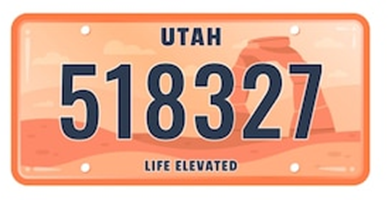
\includegraphics[width=2.18819in,height=1.11111in]{media/image2.png}
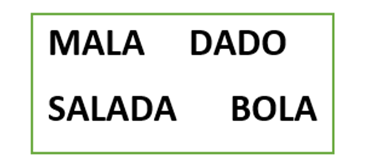
\includegraphics[width=2.03681in,height=1.04861in]{media/image3.png}
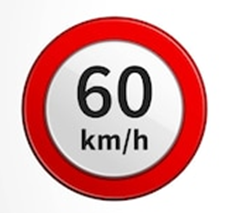
\includegraphics[width=1.20556in,height=1.11111in]{media/image4.png}

\hspace{2cm}
\includegraphics[width=0.40972in,height=0.30069in]{media/image5.png}
\hspace{4.5cm}
\includegraphics[width=0.40972in,height=0.30069in]{media/image5.png}
\hspace{3cm}
\includegraphics[width=0.40972in,height=0.30069in]{media/image5.png}
\end{figure}

\num{3} PINTE SOMENTE O QUE É USADO PARA ESCREVER AS PALAVRAS.

\begin{figure}[htpb!]
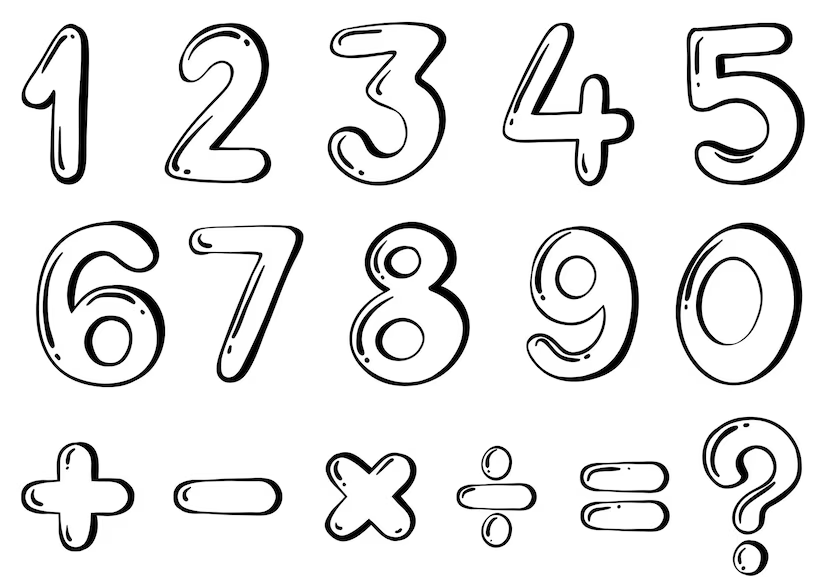
\includegraphics[width=2.23393in,height=1.58569in]{media/image6.png}
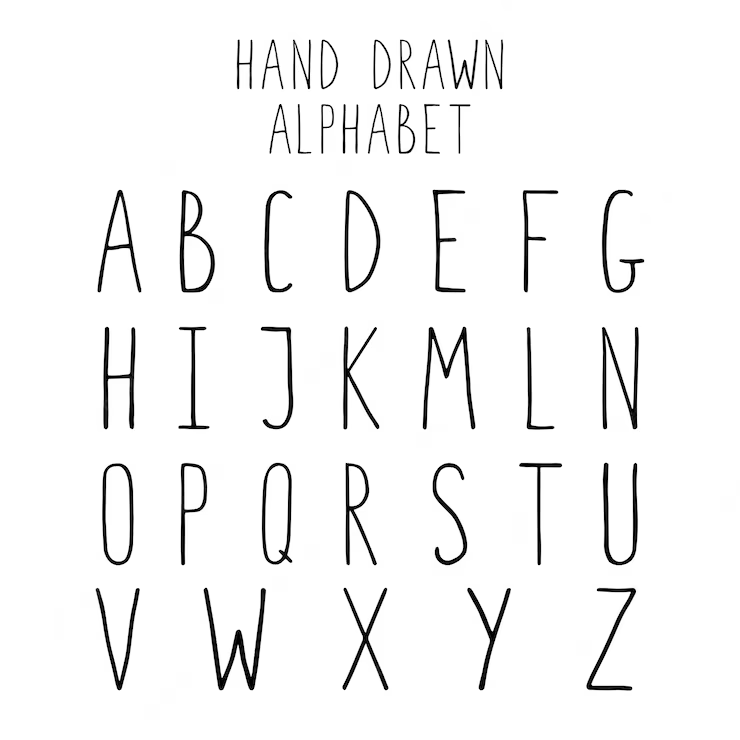
\includegraphics[width=1.96211in,height=1.66818in]{media/image7.png}
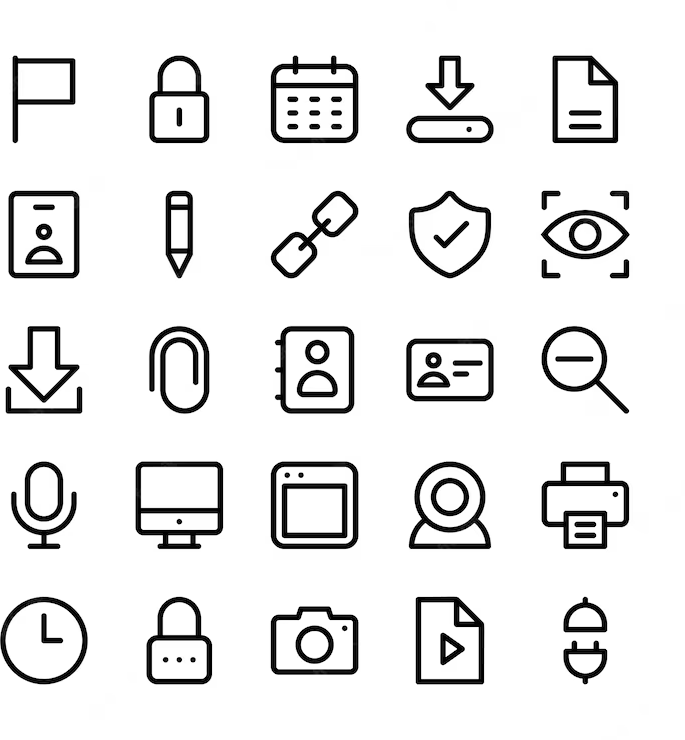
\includegraphics[width=1.56875in,height=1.56875in]{media/image8.png}
\end{figure}

%\coment{O aluno deve pintar a imagem B.}

%Colocar as imagens dentro de um quadro a b e c.

\pagebreak
\num{4} ESCREVA A PRIMEIRA LETRA DO NOME DAS FIGURAS.\bigskip

%\coment{Para essa atividade, é importante apresentar as letras do alfabeto para ensinar o som de cada uma. Leve algumas imagens e peça às crianças para formar seus nomes explorando o som das sílabas inicial, medial e final. }

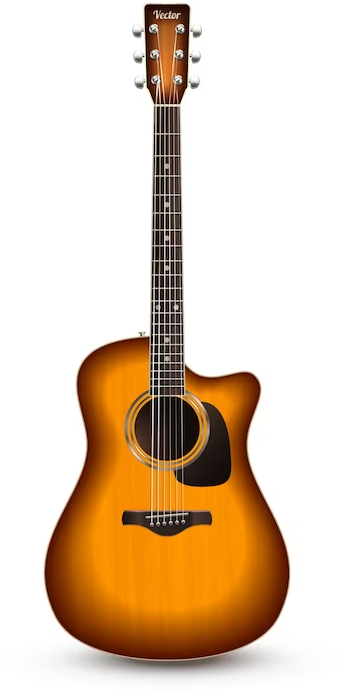
\includegraphics[width=.15\textwidth]{media/image9.png}
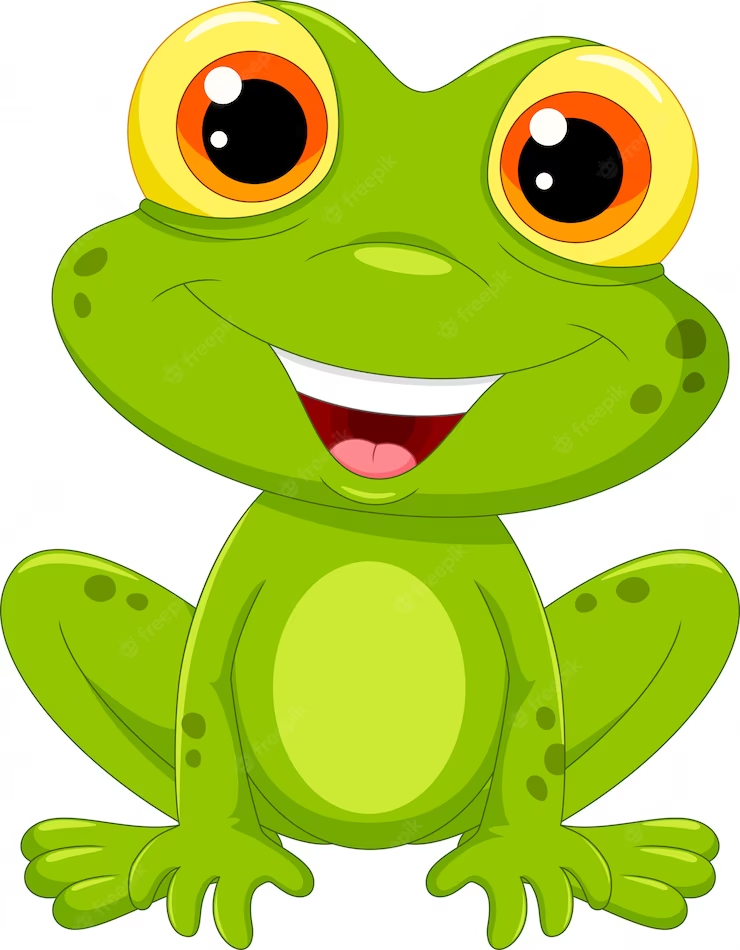
\includegraphics[width=.15\textwidth]{media/image10.png}
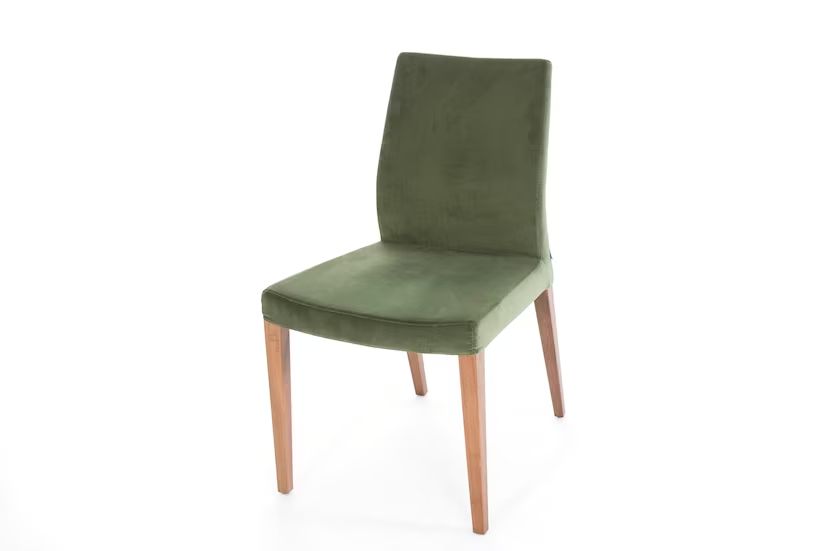
\includegraphics[width=.25\textwidth]{media/image11.png}
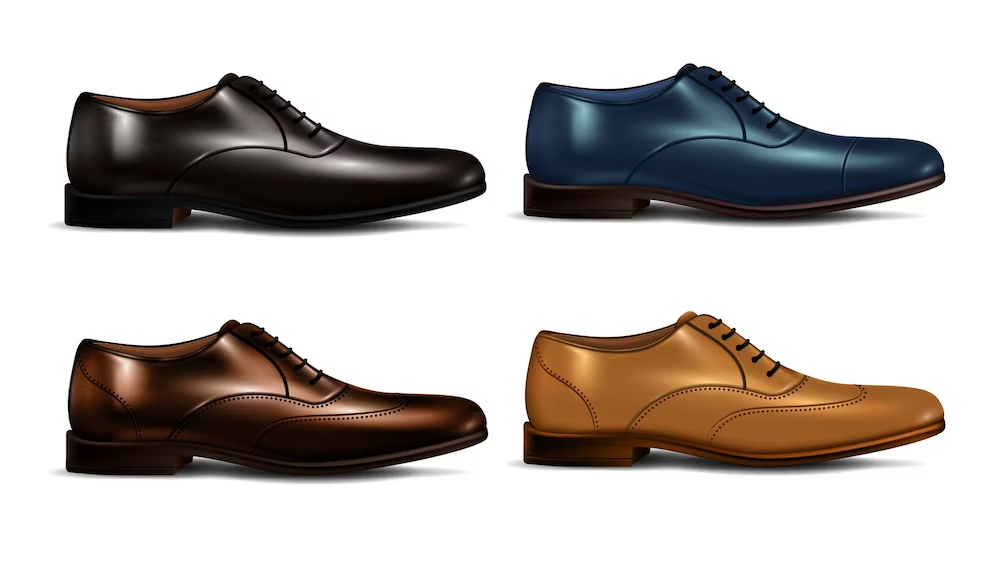
\includegraphics[width=.3\textwidth]{media/image12.png}

\hspace*{.5cm}
\includegraphics[width=0.40972in,height=0.30069in]{media/image5.png}
\hspace{1.5cm}
\includegraphics[width=0.40972in,height=0.30069in]{media/image5.png}
\hspace{2.5cm}
\includegraphics[width=0.40972in,height=0.30069in]{media/image5.png}
\hspace{2cm}
\includegraphics[width=0.40972in,height=0.30069in]{media/image5.png}

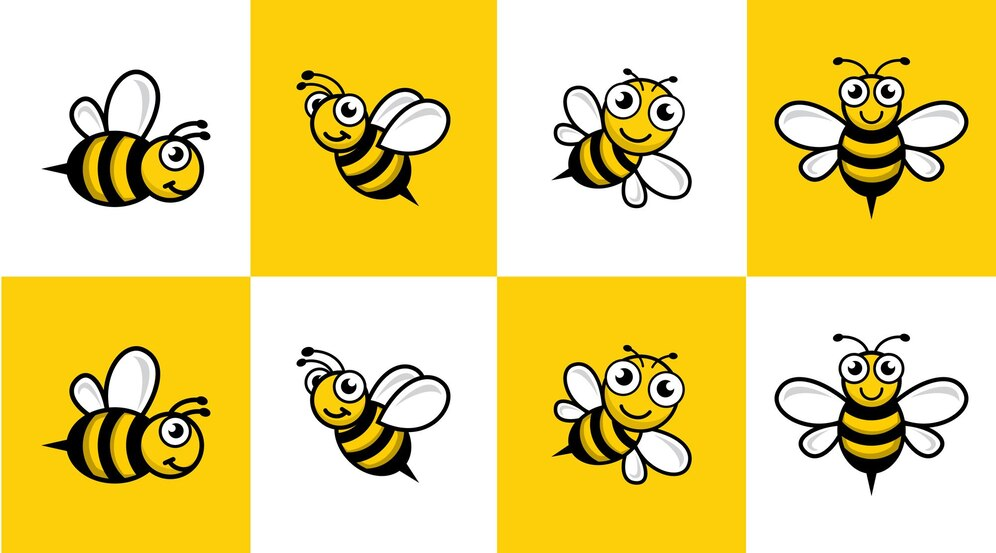
\includegraphics[width=.25\textwidth]{media/image13.png}
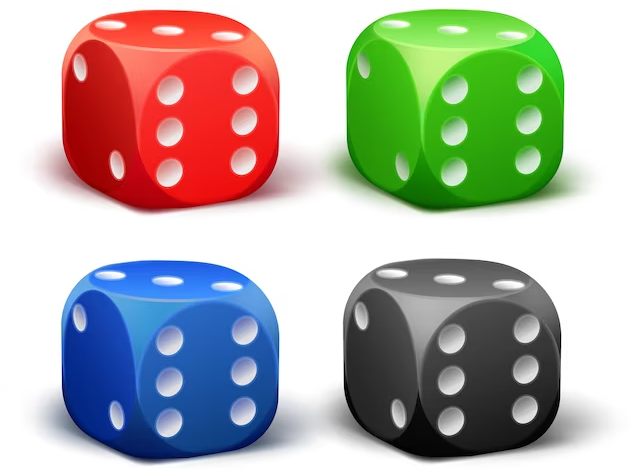
\includegraphics[width=.25\textwidth]{media/image14.png}
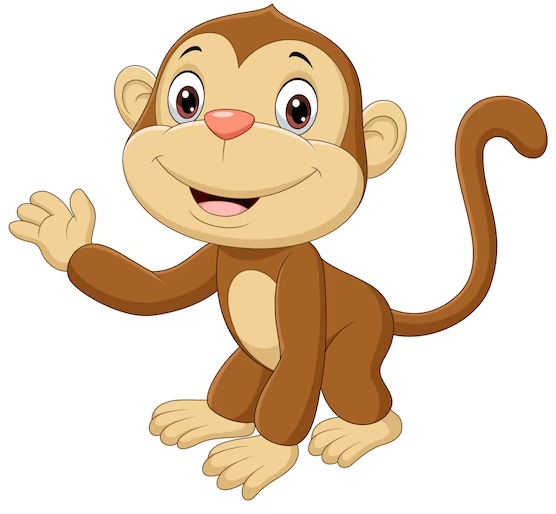
\includegraphics[width=.25\textwidth]{media/image15.png}
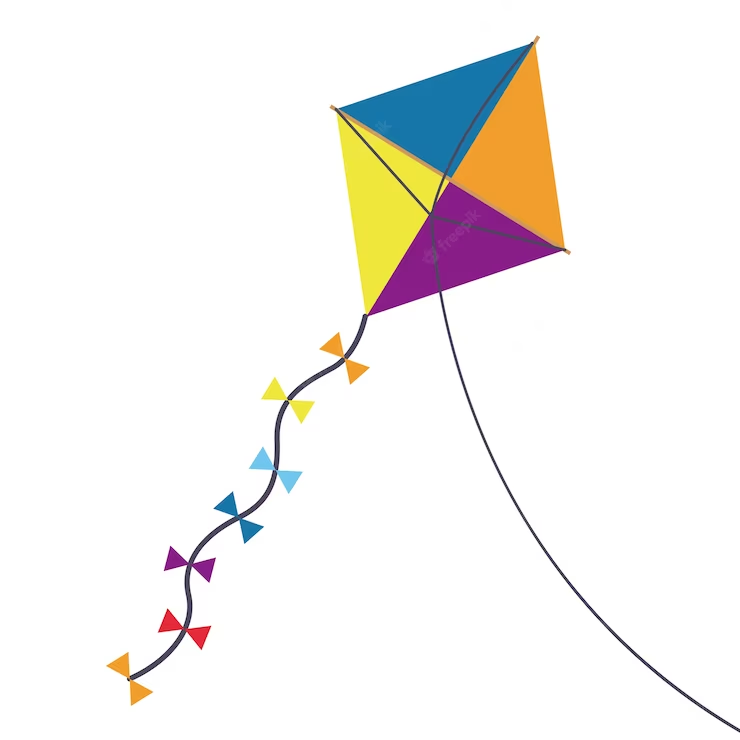
\includegraphics[width=.25\textwidth]{media/image16.png}
\hspace*{2cm}
\includegraphics[width=0.40972in,height=0.30069in]{media/image5.png}
\hspace{2.5cm}
\includegraphics[width=0.40972in,height=0.30069in]{media/image5.png}
\hspace{2.5cm}
\includegraphics[width=0.40972in,height=0.30069in]{media/image5.png}
\hspace{2.5cm}
\includegraphics[width=0.40972in,height=0.30069in]{media/image5.png}

\num{5} ESCREVA AS SÍLABAS QUE ESTÃO FALTANDO PARA COMPLETAR O NOME DO DESENHO
\bigskip

%\coment{Retome o alfabeto móvel para formar o nome das palavras, contar as letras que formam cada uma com seus respectivos sons iniciais, mediais e finais e comparar as palavras em que aparecem sons iguais. }

\begin{tabular}{lll|lll|ll|ll}
\multicolumn{3}{l|}{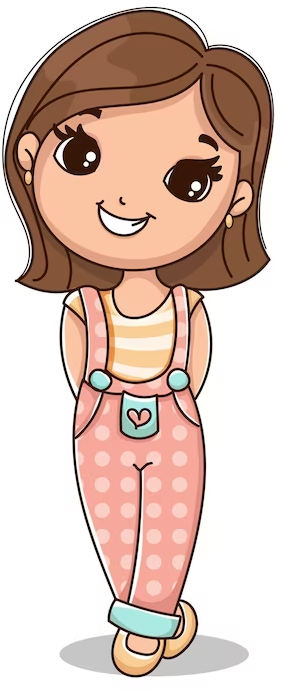
\includegraphics[width=.1\textwidth]{media/image17.png}} & \multicolumn{3}{l|}{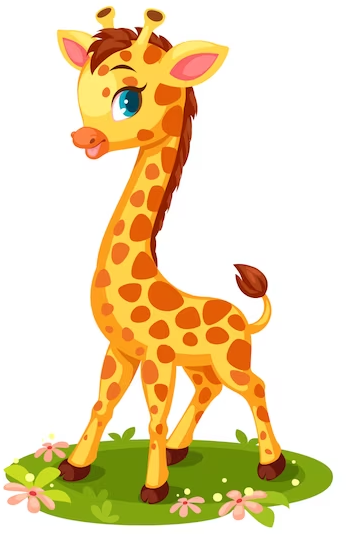
\includegraphics[width=.15\textwidth]{media/image18.png}} & \multicolumn{2}{l|}{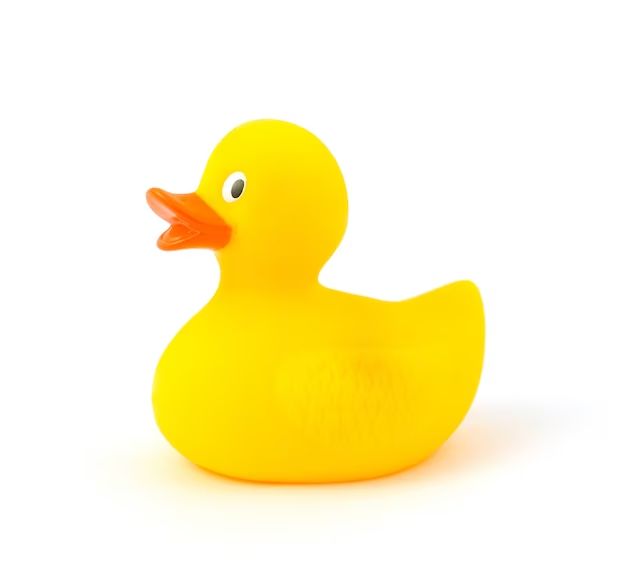
\includegraphics[width=.2\textwidth]{media/image19.png}} & \multicolumn{2}{l}{
\includegraphics[width=.3\textwidth]{media/image20.png}} \\
\multicolumn{3}{c|}{{\rosa{ME}} NI NA} & \multicolumn{3}{c|}{{\rosa{GI}} RA FA} & \multicolumn{2}{c|}{{\rosa{PA}} TO} & \multicolumn{2}{c}{{\rosa{BO}} LA}
\end{tabular}

\pagebreak

\begin{tabular}{lll|lll|ll|ll}
\multicolumn{3}{l|}{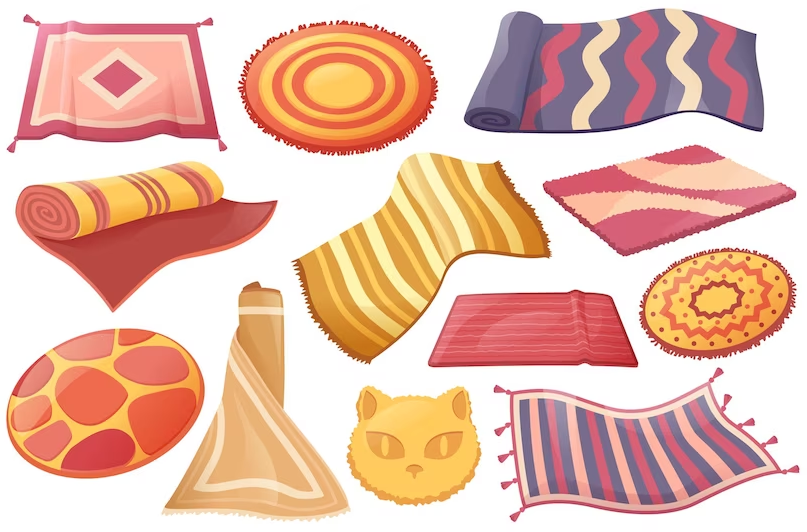
\includegraphics[width=.3\textwidth]{media/image25.png}} & \multicolumn{3}{l|}{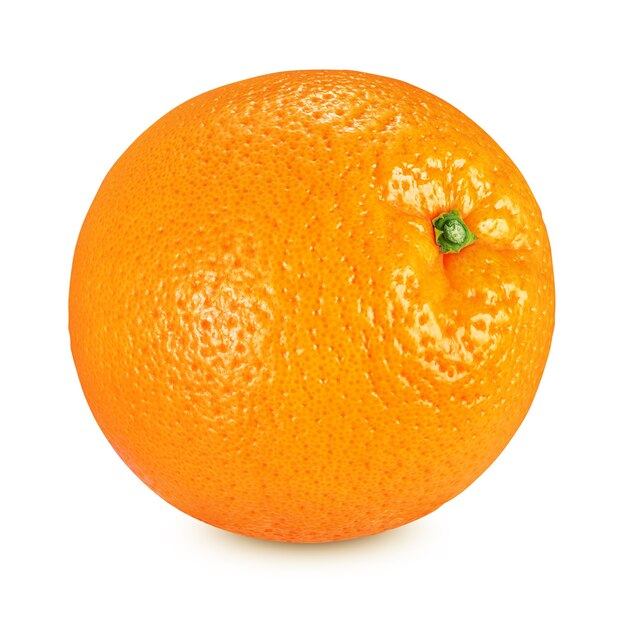
\includegraphics[width=.1\textwidth]{media/image24.png}} & \multicolumn{2}{l|}{
\includegraphics[width=.2\textwidth]{media/image23.png}} & \multicolumn{2}{l}{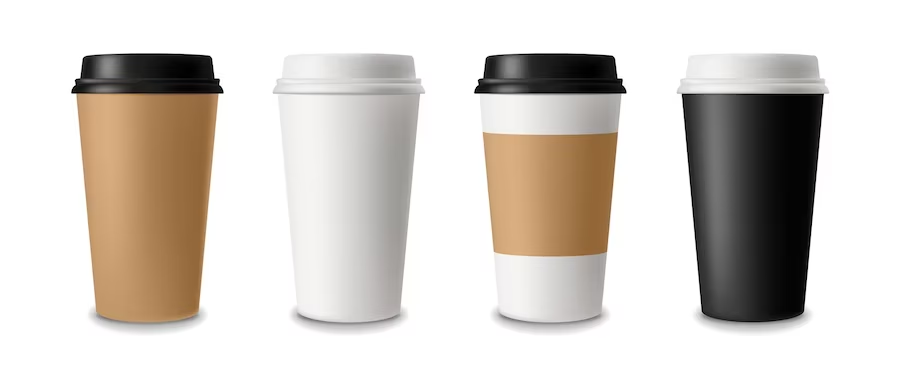
\includegraphics[width=.3\textwidth]{media/image22.png}} \\
\multicolumn{3}{c|}{{\rosa{TA}} PE TE} & \multicolumn{3}{c|}{{\rosa{LA}} RAN JA} & \multicolumn{2}{c|}{{\rosa{RA}} TO} & \multicolumn{2}{c}{{\rosa{CO}} PO}
\end{tabular}

\num{6} CONTE QUANTAS LETRAS CADA PALAVRA APRESENTA E ESCREVA EM SEGUIDA.

\begin{itemize}
\item DADO  \reduline{\mbox{ }\hfill}

\item AVIÃO \reduline{\mbox{ }\hfill}

\item CARRINHO \reduline{\mbox{ }\hfill}

\item FOCA \reduline{\mbox{ }\hfill}

\item TESOURA \reduline{\mbox{ }\hfill}

\item NAVIO \reduline{\mbox{ }\hfill}
\end{itemize}

\num{7} PINTE DE AMARELO AS PALAVRAS QUE COMEÇAM COM O MESMO SOM.

%\coment{Para essa atividade, é interessante brincar com o jogo das rimas.}

\begin{longtable}[]{@{}llll@{}}
\toprule
\textbf{JANELA} & \textbf{CANECA} & \textbf{PANELA} &
\textbf{GATO}\tabularnewline
\textbf{BANANA} & \textbf{CANELA} & \textbf{JUCA} &
\textbf{JACARÉ}\tabularnewline
\textbf{JABUTI} & \textbf{JACA} & \textbf{FADA} &
\textbf{MALA}\tabularnewline
\bottomrule
\end{longtable}

\pagebreak
\num{8} SEPARE AS SÍLABAS DOS NOMES DOS ANIMAIS
DA FAZENDO DE SEU ANTÔNIO. ESCREVA A QUANTIDADE DE PEDACINHOS NO
QUADRO
\bigskip

\begin{tabular}{l|c|c|}
\cline{2-3}
 & SÍLABAS & QUANTIDADE \\ \hline
\multicolumn{1}{|l|}{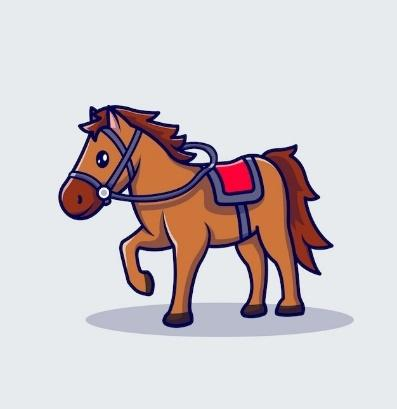
\includegraphics[width=.2\textwidth]{media/image26.jpg}} & {\rosa{CA VA LO}} & {\rosa{3}} \\ \hline
\multicolumn{1}{|l|}{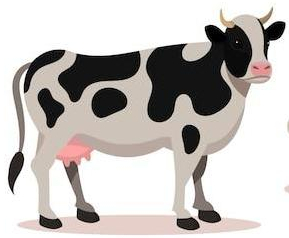
\includegraphics[width=.2\textwidth]{media/image27a.jpg}} & {\rosa{VA CA}} & {\rosa{2}} \\ \hline
\multicolumn{1}{|l|}{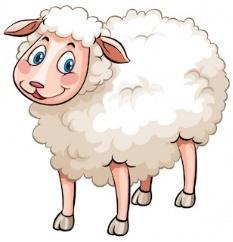
\includegraphics[width=.2\textwidth]{media/image28.jpg}} & {\rosa{O VE LHA}} & {\rosa{3}} \\ \hline
\multicolumn{1}{|l|}{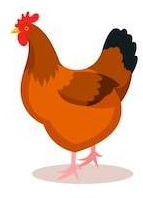
\includegraphics[width=.2\textwidth]{media/image27b.jpg}} & {\rosa{GA LI NHA}} & {\rosa{3}} \\ \hline
\multicolumn{1}{|l|}{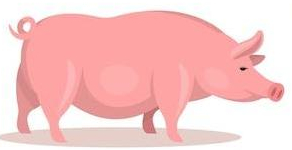
\includegraphics[width=.2\textwidth]{media/image27c.jpg}} & {\rosa{POR CO}} & {\rosa{2}} \\ \hline
\end{tabular}

%\coment{Leia as palavras com os alunos e, em seguida, convide-os a baterem palmas para observar quantas vezes abrem a boca para falar as sílabas.}

\pagebreak
\num{9} ENCONTRE E PINTE OS NOMES DOS DESENHOS NO CAÇA-PALAVRAS.

%\coment{Retome o alfabeto móvel para ajudar as crianças a formarem as palavras observando os sons finais iguais ou palavras que rimam. Em seguida, pintá-las no caça-palavras.}

\begin{figure}[htpb!]
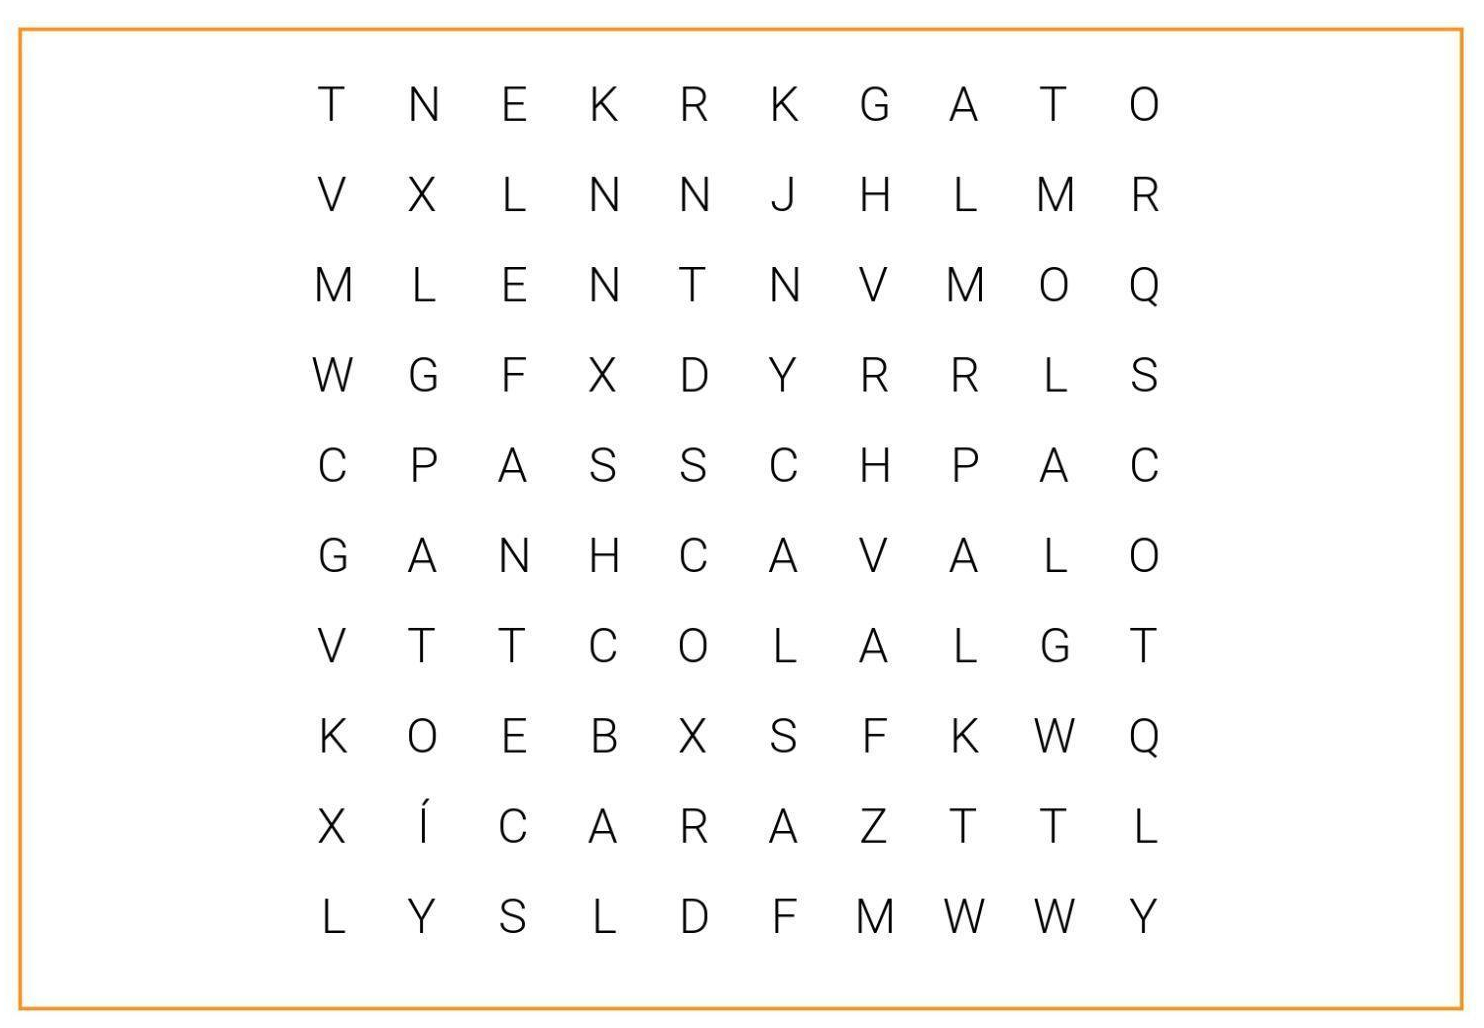
\includegraphics[width=\textwidth]{media/image29.jpg}
\end{figure}

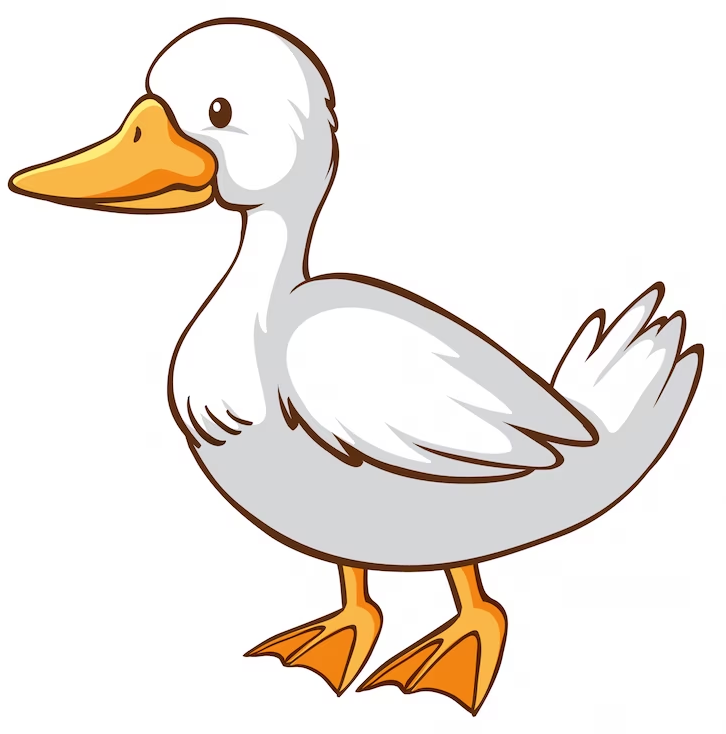
\includegraphics[width=.25\textwidth]{media/image30.png}
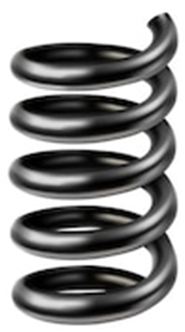
\includegraphics[width=.1\textwidth]{media/image31.png}
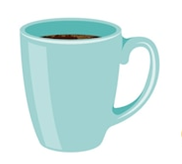
\includegraphics[width=.25\textwidth]{media/image32.png}
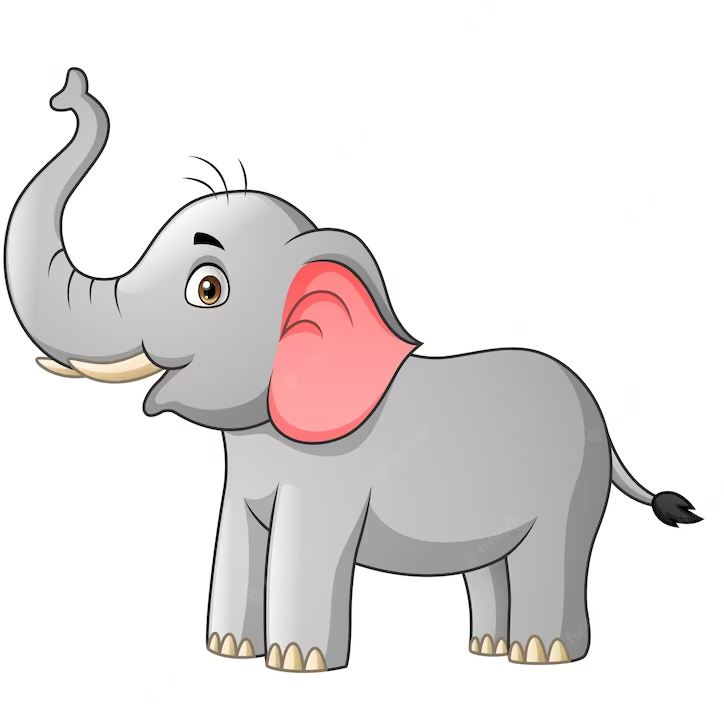
\includegraphics[width=.25\textwidth]{media/image33.png}


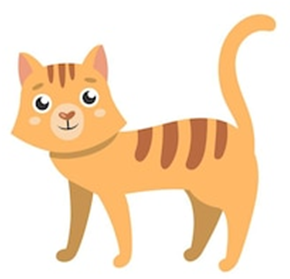
\includegraphics[width=.25\textwidth]{media/image34.png}
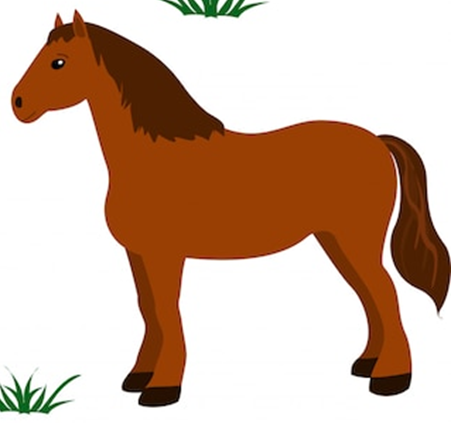
\includegraphics[width=.25\textwidth]{media/image35.png}
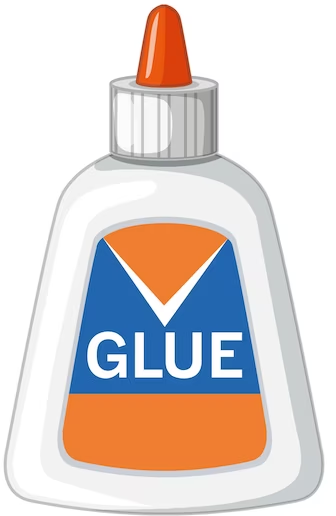
\includegraphics[width=.15\textwidth]{media/image36.png}

%Fazer um caça-palavras igual a esse.

%\coment{Resposta caça- palavras 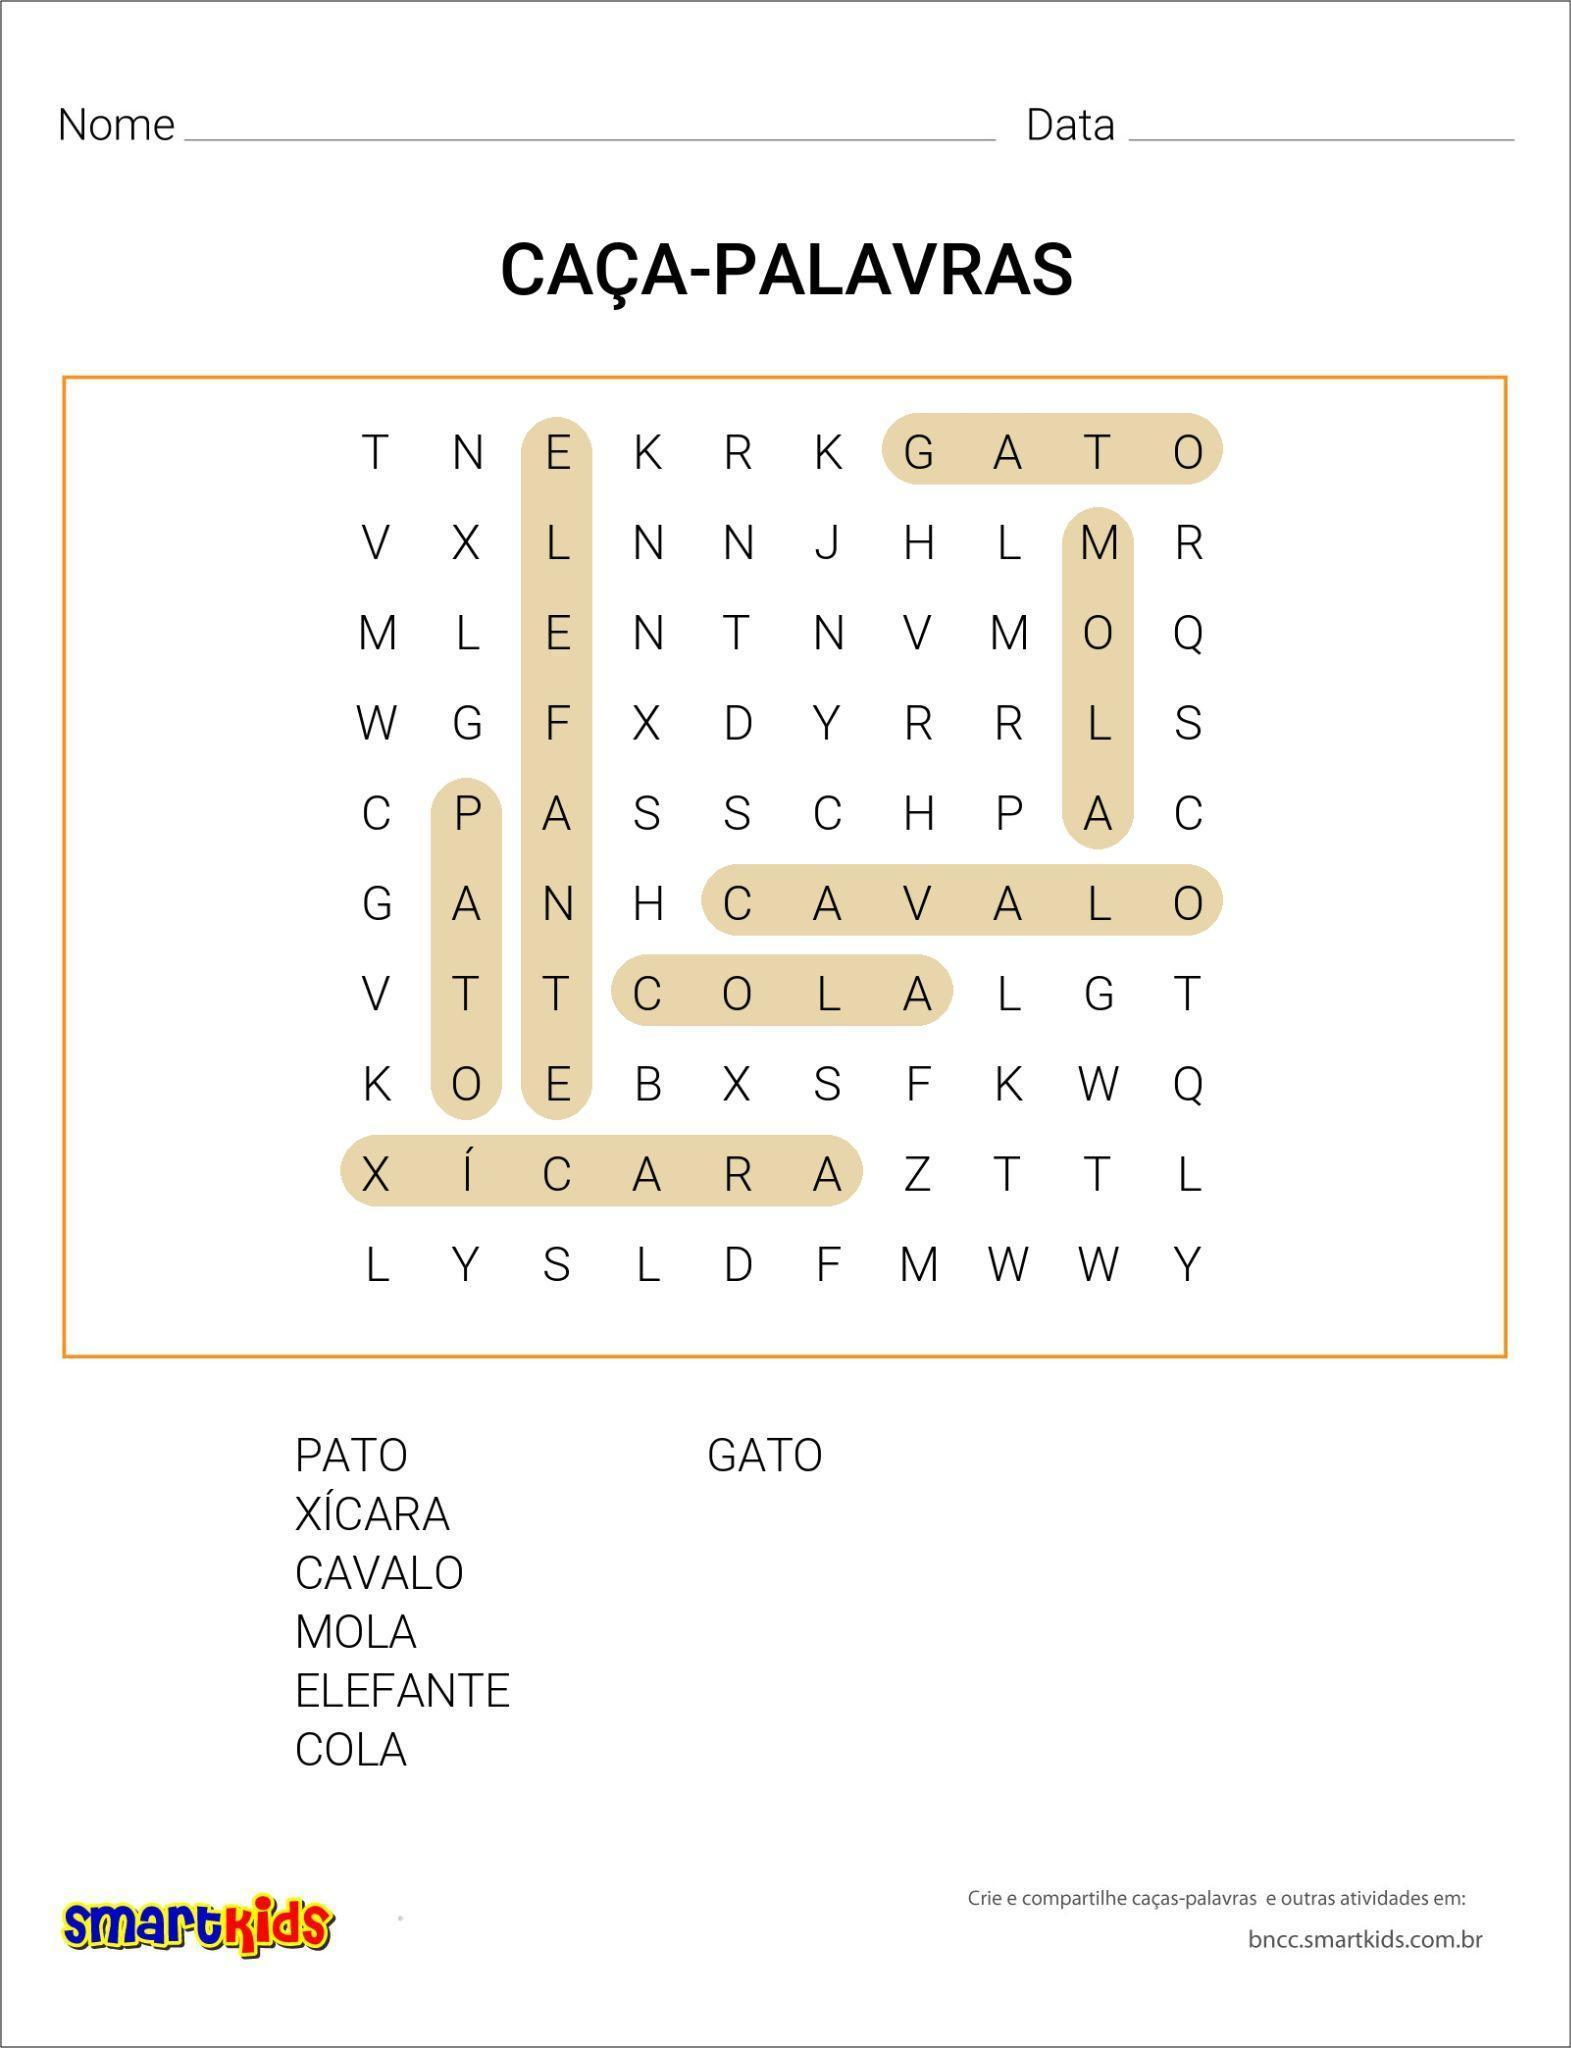
\includegraphics[width=2.13750in,height=1.44792in]{media/image37.jpg} }

\pagebreak
AGORA ESCREVA AS PALAVRAS QUE RIMAM.

\reduline{Mola e cola\hfill}
\linhas{1}


\num{9} PINTE AS PALAVRAS QUE COMEÇAM E TERMINAM COM O SOM DE VOGAL.\bigskip

\begin{tabular}{ll}
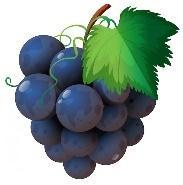
\includegraphics[width=0.83333in,height=0.84004in]{media/image38.jpg} & U V A \\
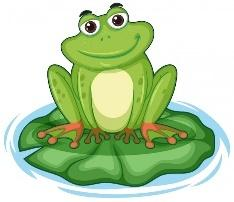
\includegraphics[width=1.06463in,height=0.91667in]{media/image39.jpg} & S A P O \\
\includegraphics[width=0.86458in,height=0.86667in]{media/image40.jpg} & Í M A \\
\includegraphics[width=1.07292in,height=0.97005in]{media/image41.jpg} & P A  T O \\
\includegraphics[width=0.85417in,height=1.14167in]{media/image42.jpg} & A N J O
\end{tabular}

\pagebreak
\num{10} LIGUE OS DESENHOS AOS SEUS RESPECTIVOS NOMES.

PANELA \hfill\includegraphics[width=.2\textwidth]{media/image43.png}

GELATINA \hfill\includegraphics[width=.15\textwidth]{media/image44.png}

PIÃO \hfill\includegraphics[width=.4\textwidth]{media/image45.jpg}

BICICLETA \hfill\includegraphics[width=.4\textwidth]{media/image46.png}

SOFÁ \hfill\includegraphics[width=.3\textwidth]{media/image48.png}

\num{11} ENCONTRE E CIRCULE O INTRUSO ENTRE AS PALAVRAS.

\begin{longtable}[]{@{}llll@{}}
\toprule
\textbf{M4ÇÃ} & \textbf{R\%TO} & \textbf{TAT\#} &
\textbf{TAPET3}\tabularnewline
\textbf{CAS7} & \textbf{MOL\%} & \textbf{BUL@} &
\textbf{DOC2}\tabularnewline
\bottomrule
\end{longtable}

AGORA ESCREVA A PALAVRA CORRETAMENTE.

\reduline{Maçâ- rato -- tatu - tapete -- casa -- mola -- bule -- doce.\hfill}
\linhas{4}

\num{12} CIRCULE O DESENHO CUJO NOME COMEÇA COM O MESMO SOM DA FIGURA EM DESTAQUE.

\begin{tabular}{l|l}
\includegraphics[width=0.81250in,height=0.75903in]{media/image49.jpg} & \includegraphics[width=.65\textwidth]{media/image50a.png} \\
\includegraphics[width=1.12431in,height=0.78125in]{media/image53.jpg} & \includegraphics[width=.65\textwidth]{media/image50b.png} \\
\includegraphics[width=1.22986in,height=0.61458in]{media/image57.jpg} & \includegraphics[width=.65\textwidth]{media/image50c.png} \\
\includegraphics[width=0.77569in,height=0.78125in]{media/image61.jpg} & \includegraphics[width=.65\textwidth]{media/image50d.png}
\end{tabular}


\num{13} TRANSCREVA A SÍLABA DO MEIO DOS NOMES DAS FIGURAS.

%\coment{Retome o alfabeto móvel para formar os nomes dos desenhos explorando os sons iniciais mediais e finais. Conte quantas vezes abrimos a boca para falar a palavra.}
\begin{center}
\begin{tabular}{lll}
\includegraphics[width=.2\textwidth]{media/image64.png} & \includegraphics[width=.2\textwidth]{media/image65.png} & \includegraphics[width=.2\textwidth]{media/image66.png} \\ \hline
\multicolumn{1}{|c|}{\rosa{NE}} & \multicolumn{1}{c|}{\rosa{TI}} & \multicolumn{1}{c|}{\rosa{VO}} \\ \hline
\end{tabular}
\end{center}

\begin{center}
\begin{tabular}{lll}
\includegraphics[width=.2\textwidth]{media/image67.png} & \includegraphics[width=.2\textwidth]{media/image68.png} & \includegraphics[width=.2\textwidth]{media/image69.png} \\ \hline
\multicolumn{1}{|c|}{\rosa{RA}} & \multicolumn{1}{c|}{\rosa{MI}} & \multicolumn{1}{c|}{\rosa{MA}} \\ \hline
\end{tabular}
\end{center}

\num{14} PINTE AS PALAVRAS QUE TERMINAM COM O MESMO SOM.

\begin{longtable}[]{@{}lll@{}}
\toprule
\textbf{TAPETE} & \textbf{POMADA} & \textbf{GILETE}\tabularnewline
\textbf{PANELA} & \textbf{TOMATE} & \textbf{JIBOIA}\tabularnewline
\textbf{JACARÉ} & \textbf{GATO} & \textbf{SALADA}\tabularnewline
\bottomrule
\end{longtable}

\num{15} OBSERVE A FIGURA E PINTE O SEU NOME.

\begin{center}
\begin{tabular}{ccc}
\multicolumn{1}{l}{\includegraphics[width=.2\textwidth]{media/image70.png}} & \multicolumn{1}{l}{\includegraphics[width=.2\textwidth]{media/image72.png} } & \multicolumn{1}{l}{\includegraphics[width=.2\textwidth]{media/image73.png}} \\ \hline
\multicolumn{1}{|c|}{COELHO} & \multicolumn{1}{c|}{MELÃO} & \multicolumn{1}{c|}{TATU} \\ \hline
\multicolumn{1}{|c|}{COBRA} & \multicolumn{1}{c|}{MACACO} & \multicolumn{1}{c|}{TELEFONE} \\ \hline
\multicolumn{1}{|c|}{ESPELHO} & \multicolumn{1}{c|}{MENINA} & \multicolumn{1}{c|}{TELEVISÃO} \\ \hline
\end{tabular}
\end{center}

\begin{center}
\begin{tabular}{ccc}
\multicolumn{1}{l}{\includegraphics[width=.2\textwidth]{media/image74.png}} & \multicolumn{1}{l}{\includegraphics[width=.2\textwidth]{media/image75.png} } & \multicolumn{1}{l}{\includegraphics[width=.2\textwidth]{media/image76.png}} \\ \hline
\multicolumn{1}{|c|}{RÉGUA} & \multicolumn{1}{c|}{ESCOLA} & \multicolumn{1}{c|}{MOLA} \\ \hline
\multicolumn{1}{|c|}{RELÓGIO} & \multicolumn{1}{c|}{ESCOVA} & \multicolumn{1}{c|}{MAMÃO} \\ \hline
\multicolumn{1}{|c|}{ÉGUA} & \multicolumn{1}{c|}{ESMALTE} & \multicolumn{1}{c|}{MALA} \\ \hline
\end{tabular}
\end{center}

\num{16} COLOQUE AS SÍLABAS EM ORDEM PARA FORMAR O NOME DAS FIGURAS.

%\coment{Para essa atividade, a utilização do alfabeto móvel poderá ser retomada.}
\begin{center}
\begin{tabular}{l|l|}
\cline{2-2}
\multirow{4}{*}{\includegraphics[width=.2\textwidth]{media/image77.png}} & CA COL CHE \\
 &  \\ \cline{2-2} 
 & \rosa{CACHECOL} \\
 &  \\ \cline{2-2}
\multirow{4}{*}{\includegraphics[width=.2\textwidth]{media/image78.png}} & PIS LÁ \\
 &  \\ \cline{2-2} 
 & \rosa{LÁPIS} \\
 &  \\ \cline{2-2}
\multirow{4}{*}{\includegraphics[width=.2\textwidth]{media/image79.jpg}} & GE TI LA \\
 &  \\ \cline{2-2} 
 & \rosa{TIGELA} \\
 &  \\ \cline{2-2}
\multirow{4}{*}{\includegraphics[width=.2\textwidth]{media/image81.png}} & CA CO MA \\
 &  \\ \cline{2-2} 
 & \rosa{MACACO} \\
 &  \\ \cline{2-2} 
\end{tabular}
\end{center}

\pagebreak


\colorsec{TREINO}

%\coment{Os três itens a seguir estão ordenados do nível mais fácil ao mais difícil. }

\num{1} FELIPE ENCONTROU ALGUMAS PLACAS GUARDADAS NO ARMÁRIO DA BIBLIOTECA. A
PLACA EM QUE SÓ APARECEM LETRAS É

\begin{escolha}
\item \includegraphics[width=.35\textwidth]{media/image82a.png}

\item \includegraphics[width=.35\textwidth]{media/image82b.png}

\item \includegraphics[width=.35\textwidth]{media/image82c.png}

\item \includegraphics[width=.35\textwidth]{media/image82d.png}
\end{escolha}
%IMAGEM ELABORADA PELO AUTOR

\num{2} OBSERVE O BRINQUEDO QUE ANA GANHOU EM UM SORTEIO.

\begin{center}
\includegraphics[width=.5\textwidth]{media/image83.png}
\end{center}

O SOM INICIAL DO NOME DO BRINQUEDO DE ANA É:

\begin{escolha}
\item PA.

\item NE.

\item GA.

\item TE.
\end{escolha}


\num{3} PEDRO ESTAVA PASSEANDO NO JARDIM DA SUA CASA E ENCONTROU UM PAPEL COM UMA ESCRITA. VEJA.

\begin{figure}[htpb!]
\centering
\includegraphics[width=.8\textwidth]{media/image84.png}
\end{figure}

%\Disponível em:\href{https://www.freepik.com/free-vector/flat-design-spring-landscape-illustrated_12239756.htm\#query=jardim\&position=2\&from_view=search\&track=sph}{\emph{https://www.freepik.com/free-vector/flat-design-spring-landscape-illustrated\_12239756.htm\#query=jardim\&position=2\&from\_view=search\&track=sph}}. Acesso em 11 de fev 2023.

QUAL PALAVRA COMEÇA COM O SOM DA SÍLABA FINAL DA PALAVRA QUE PEDRO ENCONTROU?

\begin{escolha}
\item TELEFONE

\item BONECA.

\item POMADA.

\item TAPETE.
\end{escolha}

\chapter{LENDO PALAVRAS E FRASES}
\markboth{Módulo 2}{}

\colorsec{Habilidades do SAEB}

\begin{itemize}
\item Ler palavras.

\item Escrever palavras.

\item Ler frases.
\end{itemize}

\colorsec{Habilidades da BNCC}

\begin{itemize}
\item EF01LP01, EF12LP01, EF01LP02, EF01LP13.
\end{itemize}

%\coment{Para iniciar as atividades do módulo, leve a música “Canoa Virou” escrita em um cartaz. Faça a leitura com as crianças explorando o texto. }

\conteudo{
VOCÊ CONSEGUE LER ESSA PALAVRA?

\begin{quote}
CANOA
\end{quote}

E ESSA FRASE?

\begin{quote}
A CANOA VIROU.
\end{quote}

PARA ESCREVER ESSA PALAVRA, FORAM USADAS AS LETRAS E SEUS SONS.

JÁ PARA ESCREVER ESSA FRASE, FORAM USADAS AS PALAVRAS.

PARA ESCREVER OS TEXTOS, É PRECISO USAR UM CONJUNTO DE FRASES. VEJA:}

\conteudo{
\begin{verse}
\textbf{A CANOA VIROU}

A CANOA VIROU\\
POIS DEIXARAM VIRAR\\
FOI POR CAUSA DE MARIA\\
QUE NÃO SOUBE REMAR.
\end{verse}

\begin{center}
\includegraphics[width=.25\textwidth]{media/image85.jpg}
\end{center}

\textbf{VOCÊ SABIA?}

QUANDO LEMOS E ESCREVEMOS UMA PALAVRA OU UM TEXTO, INICIAMOS DA
ESQUERDA PARA A DIREITA.

OBSERVE:

\begin{quote}
$\rightarrow$

CANOA
\end{quote}

TAMBÉM LEMOS E ESCREVEMOS DE CIMA PARA BAIXO.

OBSERVE:

\begin{quote}
$\downarrow$

A CANOA VIROU\\
POIS DEIXARAM VIRAR
\end{quote}
}

%http://www.dominiopublico.gov.br/download/texto/me000588.pdf

\colorsec{ATIVIDADES}

%\coment{Para a atividade, leve a parlenda "O macaco foi a feira" em um cartaz. Explorar a leitura de palavras, das frases e do texto, mostrado sempre como devemos iniciá-la.}

\num{1} LEIA A PALAVRA.

\begin{quote}
\textbf{MACACO}
\end{quote}

\begin{escolha}
\item ENCONTRE E ESCREVA A LETRA QUE INICIA A PALAVRA.

\reduline{Resposta: m\hfill}

\item CIRCULE A ÚLTIMA LETRA DA PALAVRA.
\end{escolha}

\num{2} AGORA LEIA A FRASE.

\begin{quote}
\textbf{O MACACO FOI A FEIRA.}
\end{quote}

\begin{escolha}
\item CIRCULE A PRIMEIRA PALAVRA DA FRASE.

\item ENCONTRE E COPIE A ÚLTIMA PALAVRA.

\reduline{Resposta: Feira\hfill}
\end{escolha}\enlargethispage{5\baselineskip}

\num{3} LEIA:

\begin{quote}
\begin{verse}
O MACACO FOI À FEIRA\\
NÃO SABIA O QUE COMPRAR\\
COMPROU UMA CADEIRA\\
PARA A COMADRE SE SENTAR
\end{verse}

\fonte{Domínio Público. ADIVINHAS, CANÇÕES, CANTIGAS DE RODA, PARLENDAS, POEMAS, QUADRINHAS E TRAVA-LÍNGUAS. Disponível em: https://bit.ly/2svTEzT. Acesso em 14 abr. 2023.}
\end{quote}
\pagebreak

\begin{escolha}
\item PINTE DE AZUL A PRIMEIRA PALAVRA DO TEXTO.

\item AGORA ESCREVA A PALAVRA QUE VOCÊ PINTOU.

\linhas{1}

\item PINTE DE VERDE A ÚTIMA PALAVRA DO TEXTO E ESCREVA NO ESPAÇO ABAIXO.

\linhas{1}
\end{escolha}

\num{4} DESENHE O ANIMAL QUE APARECE NA PARLENDA E ESCREVA O SEU NOME.

\begin{mdframed}[linewidth=2pt,linecolor=salmao,roundcorner=2pt]
\vspace{12cm}
\end{mdframed}

\pagebreak
\num{5} VAMOS CANTAR

%\coment{Cantar e dançar a música com as crianças na sala e explorar a primeira palavra do texto. Destacar suas sílabas inicial, medial e final e bater palmas para descobrir quantas sílabas tem a palavra.}

\begin{quote}
\begin{verse}
PIRULITO QUE BATE, BATE\\
PIRULITO QUE JÁ BATEU\\
QUEM GOSTA DE MIM É ELA\\
QUEM GOSTA DELA SOU EU.
\end{verse}
\fonte{Domínio Público. ADIVINHAS, CANÇÕES, CANTIGAS DE RODA, PARLENDAS, POEMAS, QUADRINHAS E TRAVA-LÍNGUAS. Disponível em: http://www.dominiopublico.gov.br/download/texto/me000588.pdf. Acesso em 14 abr. 2023.}
\end{quote}

\begin{escolha}
\item ENCONTRE E CIRCULE A PALAVRA QUE INICIA A MÚSICA.

\item COPIE A PALAVRA QUE VOCÊ PINTOU.

\reduline{Pirulito\hfill}

\item QUANTAS VEZES VOCÊ ABRE A BOCA PRA FALAR ESSA PALAVRA?

\linhas{1}

\item AGORA PINTE A ÚLTIMA PALAVRA DA MÚSICA.
\end{escolha}

\num{6} CIRCULE E COPIE A ÚLTIMA SÍLABA DOS NOMES DAS FIGURAS.

\includegraphics[width=1.22307in,height=1.24422in]{media/image86.jpg}
\includegraphics[width=1.53669in,height=1.29710in]{media/image87.jpg}
\includegraphics[width=1.09375in,height=1.09375in]{media/image88.png}
\includegraphics[width=1.03854in,height=1.20356in]{media/image89.jpg}

\begin{mdframed}[linewidth=2pt,linecolor=salmao,roundcorner=2pt]
ALFACE \hfill COROA \hfill GAIOLA \hfill FOGUEIRA
\end{mdframed}

\pagebreak
\num{7} OBSERVE A NUMERAÇÃO DE CADA ANIMAL E PREECHA A CRUZADINHA COM OS SEUS NOMES.

%\coment{Utilizar o alfabeto móvel para realizar essa atividade. Formar com as crianças os nomes dos desenhos para escrever na cruzadinha.}

\begin{figure}[htpb!]
\includegraphics[width=\textwidth]{media/image90.jpg}

\includegraphics[width=.22\textwidth]{media/image90b.jpg}
\end{figure}

\pagebreak
\num{8} ENCONTRE OS NOMES DAS FRUTAS NO CAÇA-PALAVRAS. DEPOIS, COPIE AS PALAVRAS NOS LUGARES INDICADOS.

%\coment{Utilizar o alfabeto móvel para realizar essa atividade. Formar com as crianças os nomes dos desenhos para escrever na cruzadinha.}

\begin{figure}[htpb!]
\includegraphics[width=\textwidth]{media/image97.jpg}
\end{figure}

\includegraphics[width=.3\textwidth]{media/image98.jpg}
\includegraphics[width=.3\textwidth]{media/image99.jpg}
\includegraphics[width=.3\textwidth]{media/image100.jpg}

\includegraphics[width=.2\textwidth]{media/image101.jpg}
\includegraphics[width=.2\textwidth]{media/image102.jpg}
\includegraphics[width=.3\textwidth]{media/image103.jpg}

\reduline{Respostas: banana, morango, acerola, uva, maçã.\hfill}

%RESPOSTA CAÇA-PALAVRAS
%\includegraphics[width=3.23199in,height=2.51443in]{media/image104.jpg}

\num{9} TRADUZA OS CÓDIGOS E ESCREVA PALAVRAS.

\begin{figure}[htpb!]
\includegraphics[width=\textwidth]{media/flag1.png}

\includegraphics[width=\textwidth]{media/flag2.png}
\end{figure}


\num{10} DESEMBARALHE AS PALAVRAS E FORME UMA FRASE.

\begin{longtable}[]{@{}lll@{}}
\toprule
AZUL. & MENINO & JOGOU\tabularnewline
O & BOLA & A\tabularnewline
\bottomrule
\end{longtable}

\reduline{O menino jogou a bola azul.\hfill}

\begin{longtable}[]{@{}llll@{}}
\toprule
A & BONECA & ÁGUA & CAIU\tabularnewline
NA & ALICE & DE\tabularnewline
\bottomrule
\end{longtable}

\reduline{A boneca de Alice caiu na água.\hfill}

\num{11} MARQUE UM X NAS FIGURAS CUJOS NOMES SE INICIAM COM O MESMO SOM DA PALAVRA CEBOLA.

%\coment{Levar as sílabas da palavra cebola divididas em sílabas. Formar os nomes dos desenhos com as letras móveis para fazer a comparação entre as sílabas das palavras.}

\includegraphics[width=1.36272in,height=0.72875in]{media/image105.jpg}
\includegraphics[width=0.90977in,height=1.00720in]{media/image106.jpg}
\includegraphics[width=0.98256in,height=1.40209in]{media/image107.jpg}
\includegraphics[width=1.12500in,height=1.12500in]{media/image108.jpg}
\includegraphics[width=1.13713in,height=1.09392in]{media/image109.jpg}

\num{12} COPIE A PRIMEIRA E A ÚLTIMA SÍLABA DO NOME DO DESENHO.\bigskip

\includegraphics[width=1.08333in,height=1.19792in]{media/image110.jpg}
\includegraphics[width=1.47778in,height=0.91667in]{media/image111.jpg}
\includegraphics[width=1.11458in,height=1.08403in]{media/image112.jpg}
\includegraphics[width=2.53125in,height=1.44792in]{media/image113.jpg}

\pagebreak
\num{13} ASSOCIE OS DESENHOS DE ACORDO COM OS NÚMEROS DAS PALAVRAS.

\begin{tabular}{llll}
\includegraphics[width=1.31458in,height=1.32014in]{media/image114.jpg} & \includegraphics[width=0.93056in,height=0.76042in]{media/image115.jpg} & \includegraphics[width=0.86956in,height=0.97145in]{media/image116.jpg} & \includegraphics[width=0.84722in,height=0.84722in]{media/image117.jpg} \\ \hline
\multicolumn{1}{|c|}{\rosa{6}} & \multicolumn{1}{c|}{\rosa{8}} & \multicolumn{1}{c|}{\rosa{2}} & \multicolumn{1}{c|}{\rosa{1}} \\ \hline
\includegraphics[width=0.95347in,height=0.54444in]{media/image118.jpg} & \includegraphics[width=1.00972in,height=0.84375in]{media/image119.jpg} & \includegraphics[width=0.96875in,height=0.99167in]{media/image120.jpg} & \includegraphics[width=1.30694in,height=0.88542in]{media/image121.jpg} \\ \hline
\multicolumn{1}{|c|}{\rosa{3}} & \multicolumn{1}{c|}{\rosa{7}} & \multicolumn{1}{c|}{\rosa{4}} & \multicolumn{1}{c|}{\rosa{5}} \\ \hline
 &  &  &  \\
\multicolumn{1}{c}{\begin{tabular}[c]{@{}c@{}}BAMBOLÊ\\ 1\end{tabular}} & \multicolumn{1}{c}{\begin{tabular}[c]{@{}c@{}}MACACO\\ 2\end{tabular}} & \multicolumn{1}{c}{\begin{tabular}[c]{@{}c@{}}ARMÁRIO\\ 3\end{tabular}} & \multicolumn{1}{c}{\begin{tabular}[c]{@{}c@{}}ABELHA\\ 4\end{tabular}} \\
 &  &  &  \\
\multicolumn{1}{c}{\begin{tabular}[c]{@{}c@{}}SAPATO\\ 5\end{tabular}} & \multicolumn{1}{c}{\begin{tabular}[c]{@{}c@{}}PAPAGAIO\\ 6\end{tabular}} & \multicolumn{1}{c}{\begin{tabular}[c]{@{}c@{}}ANEL\\ 7\end{tabular}} & \multicolumn{1}{c}{\begin{tabular}[c]{@{}c@{}}MANGUEIRA\\ 8\end{tabular}}
\end{tabular}


\num{14} OBSERVE A IMAGEM E ESCREVA UMA FRASE.

%\coment{Explorar as cores e formas da imagem com as crianças.}

\begin{figure}[htpb!]
\centering
\includegraphics[width=.7\textwidth]{media/image122.jpg}
\end{figure}

\reduline{As crianças brincam no parque.\hfill}
\linhas{1}

\colorsec{TREINO}

%\coment{Os três itens a seguir estão ordenados do nível mais fácil ao mais difícil. }

\num{1} VEJA A IMAGEM:

\begin{figure}[htpb!]
\centering
\includegraphics[width=.6\textwidth]{media/image123.jpg}
\end{figure}

A PRIMEIRA SÍLABA QUE FORMA O NOME DA FIGURA É

\begin{escolha}
\item TE.

\item ET.

\item PE

\item LE
\end{escolha}

\pagebreak

\num{2} LEIA FRASE.

\begin{quote}
PAULO GOSTA DE PASSEAR NO PARQUE.
\end{quote}

QUAL É A PRIMEIRA PALAVRA DA FRASE?

\begin{escolha}
\item GOSTA.

\item PAULO

\item PARQUE.

\item PASSEAR.
\end{escolha}


\num{3} LEIA

\begin{quote}
\begin{verse}
FUI AO TORORÓ\\
BEBER ÁGUA E NÃO ACHEI\\
ENCONTREI BELA MORENA\\
QUE NO TORORÓ DEIXEI.
\end{verse}
\end{quote}

A PALAVRA QUE TERMINA O TEXO É

\begin{escolha}
\item FUI.

\item QUE.

\item ACHEI.

\item DEIXE.
\end{escolha}

\chapter{ENCONTRANDO INFORMAÇÕES}
\markboth{Módulo 3}{}

\colorsec{Habilidade do SAEB }

\begin{itemize}
\item Localizar informações explícitas em textos.
\end{itemize}

\colorsec{Habilidade da BNCC}

\begin{itemize}
\item EF15LP03.
\end{itemize}
%Para iniciar o módulo, você poderá explorar o tipo do texto que será lido, destacando a oralidade e fazendo diversos questionamentos sobre as informações que estão nos textos.}

\conteudo{
VAMOS OBSERVAR A IMAGEM DO CARTAZ.\bigskip

\noindent\includegraphics[width=\textwidth]{media/image124.jpg}\bigskip

VOCÊ SABE O QUE ESSE CARTAZ ANUNCIA?

PARA RESPONDER À PERGUNTA, É NECESSÁRIO BUSCAR AS INFORMAÇÕES NO TEXTO.}

\conteudo{
ELE ESTÁ ANUNCIANDO A CAMPANHA DE VACINAÇÃO CONTRA A GRIPE INFLUENZA, QUE ACONTECERÁ ENTRE OS DIAS 10 DE ABRIL E 31 DE MAIO. 

VEJA ESSE OUTRO TEXTO

\begin{center}
\includegraphics[width=.6\textwidth]{media/image125.jpg}
\end{center}

\textbf{A CASINHA DA VOVÓ}

\begin{verse}
A CASINHA DA VOVÓ\\
\emph{CERCADINHA DE CIPÓ}\\
O CAFÉ ESTÁ DEMORANDO\\
COM CERTEZA NÃO TEM PÓ.\\
COMO É A CASA DA VOVÓ?\\
A CASA DA VOVÓ É CERCADINHA DE SIPÓ.
\end{verse}

VEJA QUE ESSA INFORMAÇÃO APARECE NO TEXTO.

FIQUE LIGADO PARA LOCALIZAR INFORMAÇÕES EXPLICITAS EM TEXTO BASTA LER COM
ATENÇÃO POIS ELA VAI ESTÁ LÁ BEM CLARA NO TEXTO COLOCAR EM UM BOX AO
LADO DA PÁGINA.
}

\colorsec{ATIVIDADES}

%\coment{Para realizar as atividades a seguir, você poderá fazer a leitura com os alunos e explorar bastante a oralidade dos diferentes tipos de textos. }

\includegraphics[width=2.02153in,height=2.05208in]{media/image126.jpg}

LEIA O TEXTO.

\begin{quote}
\textbf{POMBINHA BRANCA}

\begin{verse}
POMBINHA BRANCA\\
O QUE ESTÁ FAZENDO\\
LAVANDO A ROUPA\\
DO CASAMENTO.
\end{verse}

\fonte{Domínio Público. ADIVINHAS, CANÇÕES, CANTIGAS DE RODA, PARLENDAS, POEMAS, QUADRINHAS E TRAVA-LÍNGUAS. Disponível em: http://www.dominiopublico.gov.br/download/texto/me000588.pdf. Acesso em 14 abr. 2023}
\end{quote}

%https://www.freepik.com/free-vector/hand-drawn-dove-outline-illustration\_22340867.htm\#query=POMBA\&position=6\&from\_view=search\&track=sph

\num{1} ENCONTRE E PINTE O TÍTULO DO TEXTO COM A COR VERDE.

\num{2} QUAL É A COR DA POMBINHA?

\reduline{Branca\hfill}

\num{3} O QUE A POMBINHA ESTÁ FAZENDO?

\reduline{Lavando roupa\hfill}

\pagebreak
LEIA AS INFORMAÇÕES DO CARTAZ.

\begin{figure}[htpb!]
\centering
\includegraphics[width=.8\textwidth]{media/image127.jpg}
\end{figure}

AGORA, RESPONDA:

\num{4} A QUAL DOENÇA O CARTAZ SE REFERE?

\reduline{À dengue\hfill}

\num{5} QUAL É O PEDIDO ESCRITO NO CARTAZ?

\reduline{Elimine os criadouros do mosquito da dengue.\hfill}

\num{6} CIRCULE NO CARTAZ ALGUNS CUIDADOS PARA COMBATER A DENGUE.

\coment{O aluno deve circular as imagens no cartaz.}

\pagebreak
LEIA COM ATENÇÃO

\begin{minipage}{.7\textwidth}
\begin{verse}
\textbf{MEIGUICE}\\
(ADELINA LOPES VIEIRA)

DERAM À LINDA CLARISSE\\
UMA GATINHA MIMOSA,\\
TÃO BRANCA, TÃO CARINHOSA,\\
TÃO ENGRAÇADA, TÃO MANSA\\
QUE A ENCANTADORA CRIANÇA\\
POR NOME LHE PÔS --- MEIGUICE.
\end{verse}
\end{minipage}
\begin{minipage}{.3\textwidth}
\includegraphics[width=2.83472in,height=2.19792in]{media/image128.jpg}
\end{minipage}

\num{7} O QUE CLARISSE GANHOU?

\reduline{Uma gatinha.\hfill}

\num{8} COMO ERA A GATINHA DE CLARISSE?

\reduline{Uma gatinha mimosa, branca, carinhosa, engraçada e mansa.\hfill}

\num{9} ENCONTRE NO TEXTO O NOME QUE CLARISSE DEU PARA SUA GATINHA.

\reduline{Meiguice.\hfill}

\num{10} COMO VOCÊ IMAGINA A GATINHA DE CLARISSE? DESENHE AQUI.

\begin{mdframed}[linewidth=2pt,linecolor=salmao,roundcorner=2pt]
\vspace{3cm}
\coment{Resposta pessoal.}
\end{mdframed}

LEIA O TEXTO

\begin{minipage}{.8\textwidth}
\begin{verse}
\textbf{PINTINHO}

MEU PINTINHO AMARELINHO\\
CATA AQUI NA MINHA MÃO,\\
NA MINHA MÃO.\\
QUANDO QUER COMER BICHINHO\\
COM SEU PEZINHO\\
ELE CISCA O CHÃO.\\
ELE BATE AS ASAS\\
ELE FAZ PIU-PIU\\
MAS TEM MUITO MEDO DO GAVIÃO.

\end{verse}
\end{minipage}
\begin{minipage}{.2\textwidth}
\includegraphics[width=\textwidth]{media/image129.png}
\end{minipage}
\fonte{Domínio Público. ADIVINHAS, CANÇÕES, CANTIGAS DE RODA, PARLENDAS, POEMAS, QUADRINHAS E TRAVA-LÍNGUAS. Disponível em: http://www.dominiopublico.gov.br/download/texto/me000588.pdf. Acesso em 14 abr. 2023. }

\num{11} ENCONTRE E CIRCULE O TÍTULO DO TEXTO

\num{12} PINTE A COR DO PINTINHO NO TEXTO.

\num{13} O QUE O PINTINHO FAZ QUANDO QUER COMER BICHINHOS?

\reduline{Com seu pezinho, ele cisca o chão.\hfill}
\linhas{2}

\num{14} DE QUEM O PINTINHO TEM MEDO?

\reduline{Do gavião.\hfill}
\linhas{2}

\pagebreak
LEIA


\begin{quote}
\includegraphics[width=.7\textwidth]{media/image130.jpg}

\textbf{BOLO DE IOGURTE}

\begin{flushleft}
\textbf{INGREDIENTES:}\\
3 OVOS\\
1 COPO DE IOGURTE NATURAL\\
1 COPO DE ÓLEO (USE O COPO DE IOGURTE PARA OBTER A QUANTIDADE CERTA)\\
1 ½ XÍCARA DE CHÁ DE AÇÚCAR REFINADO\\
2 XÍCARAS CHÁ DE FARINHA DE TRIGO\\
1 COLHER DE SOPA DE FERMENTO

\textbf{MODO DE PREPARO:}

COM A SUPERVISÃO DE UM ADULTO, COMO PROFESSOR(A), SEUS PAIS OU RESPONSÁVEIS, COLOQUE OS OVOS NO LIQUIDIFICADOR E BATA. ACRESCENTE O IOGURTE E O ÓLEO
E DÊ UM LEVE PULSAR. INCLUA O AÇÚCAR E BATA MAIS UM POUCO. PONHA A
FARINHA EM UMA TIGELA...
\end{flushleft}

\fonte{G1. Bolo de iogurte: fácil de fazer, bonito e muito gostoso.
em: \emph{https://g1.globo.com/sao-paulo/sorocaba-jundiai/nosso-campo/noticia/2016/04/bolo-de-iogurte-facil-de-fazer-bonito-e-muito-gostoso.html. Acesso em:}
12 de fev. 2023.}
\end{quote}

\num{15} QUAL É O NOME DA RECEITA?

\reduline{Bolo de iogurte.\hfill}

\num{16} AGORA, ESCREVA O NOME DE DOIS INGREDIENTES USADOS PARA FAZER O BOLO.

\reduline{Ovo e iogurte, por exemplo.\hfill}

\num{17} ESCREVA O NOME DE UM UTENSÍLIO USADO PARA FAZER A RECEITA.

\reduline{Uma xícara, por exemplo.\hfill}

LEIA

\begin{center}
\includegraphics[width=.5\textwidth]{media/image131.png}
\end{center}

\num{18} QUAL É A CAMPANHA RETRATADA NO CARTAZ?

\reduline{Vacinação contra a raiva.\hfill}

\num{19} PARA QUEM É INDICADA ESSA VACINAÇÃO?

\reduline{Para cães e gatos.\hfill}

\num{20} QUAL É O PERÍODO EM QUE A CAMPANHA OCORRERÁ?

\reduline{17/08 a 17/09.\hfill}

\pagebreak
\colorsec{TREINO}

%\coment{Os três itens a seguir estão ordenados do nível mais fácil ao mais difícil. }

\num{1} LEIA:

\textbf{AS BORBOLETAS}

\begin{verse}
BRANCAS\\
AZUIS\\
AMARELAS\\
E PRETAS\\
BRINCAM\\
NA PAZ\\
AS BELAS\\
BORBOLETAS\\
BORBOLETAS BRANCAS\\
SÃO ALEGRES E FRANCAS\\
BORBOLETAS AZUIS\\
GOSTAM MUITO DE LUZ.\\
AS AMARELINHAS\\
SÃO TÃO BONITINHAS!\\
E AS PRETAS, ENTÃO\ldots{}\\
OH QUE ESCURIDÃO!
\end{verse}

\fonte{Domínio Público. ADIVINHAS, CANÇÕES, CANTIGAS DE RODA, PARLENDAS, POEMAS, QUADRINHAS E TRAVA-LÍNGUAS. Disponível em: \emph{http://www.dominiopublico.gov.br/download/texto/me000588.pdf}.
Acesso em: 14 abr. 2023.}

QUAL É A COR DA BORBOLETA QUE GOSTA DE LUZ?

\begin{escolha}
\item
  AZUL.
\item
  PRETA.
\item
  BRANCA.
\item
  AMARELA.
\end{escolha}

\num{2} LEIA OS INGREDIENTES DE UMA RECEITA.

\begin{quote}
\textbf{INGREDIENTES:}\\

\begin{flushleft}
6 FATIAS DE PÃO INTEGRAL OU 3 MINI BAGUETES DE FARINHA INTEGRAL\\
6 COLHERES (DE SOPA) DE QUEIJO RICOTA\\
200 G LEGUMES (CENOURA COZIDA, ERVILHA, MILHO VERDE, BATATA)\\
3 FOLHAS GRANDES RASGADAS DE ALFACE AMERICANA\\
15 G PEPINO CORTADO EM FATIAS\\
100 ML IOGURTE NATURAL
\end{flushleft}

\fonte{G1. Aprenda a preparar três tipos de sanduíche para o verão. Disponível em: \emph{https://g1.globo.com/minas-gerais/noticia/2015/01/aprenda-preparar-tres-tipos-de-sanduiche-para-o-verao.html.} Acesso em: 12 fev. 2023.}
\end{quote}

O INGREDIENTE QUE VAI SER USADO NA QUANTIDADE DE 6 FATIAS É

\begin{escolha}
\item PÃO.

\item QUEIJO.

\item PEPINO.

\item CENOURA.
\end{escolha}

\pagebreak
\num{3}

\begin{quote}
\begin{verse}
\textbf{A FOCA}\\
RIO DE JANEIRO, 1970

QUER VER A FOCA\\
FICAR FELIZ?\\
É PÔR UMA BOLA\\
NO SEU NARIZ.

QUER VER A FOCA\\
BATER PALMINHA?\\
É DAR A ELA\\
UMA SARDINHA.

QUER VER A FOCA\\
FAZER UMA BRIGA?\\
É ESPETAR ELA\\
BEM NA BARRIGA!
\end{verse}

\fonte{Prefeitura de Bauru. A Foca. Disponível em: \emph{https://tinyurl.com/y5mzt3x8}. Acesso em: 14 abr. 2023.}
\end{quote}

O QUE FAZ A FOCA BATER PALMINHA?

\begin{escolha}
\item PÔR UMA BOLA NO SEU NARIZ.

\item ESPETAR BEM NA BARRIGA.

\item DAR UMA SARDINHA.

\item FAZER UMA BRIGA.
\end{escolha}

\chapter{PARA QUE SERVE ESSE TEXTO?}
\markboth{Módulo 4}{}

\colorsec{Habilidade do SAEB}

\begin{itemize}
\item Reconhecer a finalidade de um texto.
\end{itemize}

\colorsec{Habilidade da BNCC}

\begin{itemize}
\item EF15LP01.
\end{itemize}
%Para iniciar o módulo, apresente os textos e pergunte aos alunos se conhecem algum deles. Em seguida, explique a função de cada texto.}

\conteudo{
VOCÊ SABE O QUE É UM TEXTO?

UM TEXTO É UM CONJUNTO DE PALAVRAS COM LINGUAGEM E ESTRUTURA PRÓPRIAS E QUE PODE SER UTILIZADO COM FUNÇÕES DIFERENTES.

EXISTEM VÁRIOS TIPOS DE TEXTOS. VEJA ALGUNS DELES E SUAS FUNÇÕES.

\textbf{CONVITE:} SERVE PARA FAZER UM CONVITE. 

\begin{center}
\noindent\includegraphics[width=.6\textwidth]{media/image132.jpg}
\end{center}
}

\conteudo{
\textbf{RECEITA:} SERVE PARA ENSINAR A PREPARAR UM PRATO.\bigskip

\noindent\includegraphics[width=\textwidth]{media/image134.png}\bigskip

\textbf{NOTÍCIA:} SERVE PARA INFORMAR

\begin{quote}
Menino de 5 anos é brasileiro mais novo a entrar para clube mundial de pessoas com alto QI.
\end{quote}

\textbf{TIRINHA:} SERVE PARA DIVERTIR\smallskip

\noindent\includegraphics[width=\textwidth]{media/image136.png}
}

\conteudo{
\textbf{LISTA:} SERVE PARA ORGANIZAR UMA INFORMAÇÕES.

LISTA DE COMPRAS

\begin{enumerate}
\item CARNE
\item ARROZ
\item AÇÚCAR
\item ÓLEO
\item FEIJÃO
\item FARINHA
\item MACARRÃO
\item BISCOITO
\end{enumerate}
}

\pagebreak
\colorsec{ATIVIDADES}

\num{1} TIA NINA VAI APRENDER A FAZER UM PRATO PARA O ALMOÇO. QUAL TEXTO ELA DEVE USAR? MARQUE COM UM X.

\includegraphics[width=.5\textwidth]{media/image137.png}
\includegraphics[width=.5\textwidth]{media/image138.png}

\includegraphics[width=.5\textwidth]{media/image139.png}
\includegraphics[width=.5\textwidth]{media/image140.png}

\num{2} ENCONTRE E CIRCULE O TEXTO QUE SERVE PARA INFORMAR OS LEITORES. 

\includegraphics[width=.3\textwidth]{media/image141.png}
\includegraphics[width=.3\textwidth]{media/image142.png}
\includegraphics[width=.3\textwidth]{media/image143.png}

\includegraphics[width=.3\textwidth]{media/image145.png}
\includegraphics[width=.3\textwidth]{media/image147.png}
\includegraphics[width=.3\textwidth]{media/image152.png}

\bigskip
OBSERVE O TEXTO.

\begin{quote}
\includegraphics[width=.8\textwidth]{media/image153.jpg}

\textbf{BOLO DE CENOURA}
\end{quote}

\begin{quote}
\begin{flushleft}
INGREDIENTES\\
4 OVOS\\
1 XÍCARA DE ÓLEO\\
3 CENOURAS MÉDIAS DESCASCADAS E PICADAS\\
2 XÍCARAS DE AÇÚCAR\\
2 XÍCARAS DE FARINHA DE TRIGO\\
1 COLHER DE SOPA DE FERMENTO

MODO DE PREPARAR

\begin{itemize}
\item
  MISTURE A FARINHA DE TRIGO, O AÇÚCAR E O FERMENTO NUMA TIGELA.

\item
  BATA OS OVOS, O ÓLEO E AS CENOURAS NO LIQUIDIFICADOR.

\item
  MISTURE O QUE FOI BATIDO NO LIQUIDIFICADOR AOS INGREDIENTES QUE ESTÃO NA TIGELA.
\end{itemize}
\end{flushleft}

\fonte{https://portal.educacao.go.gov.br/wp-content/uploads/2021/08/Atividade-12-1-o-ano-Lingua-Portuguesa-Tema-Receitas-FIinalidade-do-texto-Composicao-do-texto-Professor.pdf. Acesso em 18 Fev 2023.}
\end{quote}

\num{3} COMO SE CHAMA ESSE TIPO DE TEXTO?

\reduline{Receita.\hfill}

\num{4} PARA QUE SERVE ESSE TIPO DE TEXTO?

\reduline{A função de uma receita é ensinar o leitor a preparar um prato.\hfill}

\num{5} ESCREVA OS NOMES DE DOIS INGREDIENTES DA RECEITA.

\reduline{Cenoura e açúcar, por exemplo.\hfill}

\pagebreak
\num{6} CONSTRUA UM TEXTO PARA ORGANIZAR AS COMPRAS DE FRUTAS DO MÊS. ESCREVA O TIPO DE TEXTO NO TOPO.

\reduline{Resposta pessoal.\hfill}
\linhas{4}

\num{7} PREENCHA A CRUZADINHA DE ACORDO COM AS CARACTERÍSTICAS DE CADA TEXTO.

\begin{figure}[htpb!]
\centering
\includegraphics[width=.7\textwidth]{media/image155.png}
\end{figure}

\coment{1- Receita. 2- Bilhete. 3- Convite. 4- Tirinha. 5- Notícia. 6- Cartaz.}

\pagebreak
LEIA ESSE TEXTO.

\begin{figure}[htpb!]
\centering
\includegraphics[width=\textwidth]{media/image156.png}
\end{figure}

%\fonte{Disponível em: \emph{https://riovermelho.mg.gov.br/rio-vermelho-iniciara-vacinacao-de-criancas/} Acesso em: 18 fev. 2023.}

\num{8} COMO É CHAMADO ESSE TEXTO?


\reduline{Cartaz.\hfill}

\num{9} PARA QUE ELE SERVE?

\reduline{Informar sobre as vacinas.\hfill}

\num{10} A QUAL GRUPO ELE É DESTINADO?

\reduline{Para as crianças.\hfill}

\pagebreak
\colorsec{TREINO}

%\coment{Os três itens a seguir estão ordenados do nível mais fácil ao mais difícil. }

\num{1} OBSERVE O TEXTO.

\begin{figure}[htpb!]
\centering
\includegraphics[width=.9\textwidth]{media/image157.png}
%\fonte{Elaborado pela autora}
\end{figure}

ESTE TEXTO É

\begin{escolha}
\item UMA CARTA.

\item UMA RECEITA.

\item UM CONVITE.

\item UMA AGENDA.
\end{escolha}

\pagebreak
\num{2} LEIA O TEXTO:

\begin{figure}[htpb!]
\centering
\includegraphics[width=\textwidth]{media/image158.jpg}
%\fonte{Disponível em: https://www.boituva.sp.gov.br/imprensa/noticias/dia-das-criancas-no-centro-de-eventos. Acesso em: 18 fev. 2023.}
\end{figure}

A FINALIDADE DO TEXTO É

\begin{escolha}
\item ORGANIZAR TAREFAS.

\item ENSINAR UMA RECEITA.

\item INFORMAR UM EVENTO.

\item CONTAR UMA HISTÓRIA.
\end{escolha}

\pagebreak
\num{3} LEIA:

\textbf{SALADA DE FRUTAS}

\includegraphics[width=2.90350in,height=1.63264in]{media/image159.jpg}

INGREDIENTES\\
3 BANANAS\\
1 MAMÃO PEQUENO\\
3 MAÇÃS\\
4 LARANJAS\\
METADE DE 1 ABACAXI\medskip

MODO DE PREPARAR

\begin{itemize}
\item
  LAVE AS FRUTA.
\item
  DESCASQUE E PIQUE TODAS BEM PEQUENININHAS, COM A EXCEÇÃO DA LARANJA.
\item
  DESCASQUE E PIQUE SÓ 2 LARANJAS.
\item
  COM AS OUTRAS 2 LARANJAS, FAÇA UM SUCO E DESPEJE POR CIMA DA SALADA.
\end{itemize}

\fonte{Secretaria de Estado da Educação de Goiás. Bolo de Cenoura. Disponível em:
\emph{https://portal.educacao.go.gov.br/wp-content/uploads/2021/08/Atividade-12-1-o-ano-Lingua-Portuguesa-Tema-Receitas-FIinalidade-do-texto-Composicao-do-texto-Professor.pdf}. Acesso em: 18 fev. 2023.}

%https://www.freepik.com/free-photo/mixed-assorted-fruits\_4124941.htm\#query=salada\%20de\%20frutas\&position=6\&from\_view=search\&track=ais

ESTE TEXTO SERVE PARA

\begin{escolha}
\item ENSINAR A PREPARAR UMA COMIDA.

\item INFORMAR AS VITAMINAS DAS FRUTAS.

\item FAZER A PROPAGANDA DE UMA COMIDA.

\item FALAR SOBRE OS NUTRIENTES DE UM SUCO.
\end{escolha}

\chapter{COMPREENDER O TEXTO}
\markboth{Módulo 5}{}

\colorsec{Habilidade do SAEB}

\begin{itemize}
\item Inferir o assunto de um texto.
\end{itemize}

%\coment{Para realizar as atividades deste módulo, leia todos os textos com os alunos, explorando seu tipo, título, personagens e as informações contidas neles e levantado hipóteses sobre os assuntos.}

\conteudo{
COMO VOCÊ ACHA QUE UM TEXTO É FORMADO?

UM TEXTO É FORMADO POR PALAVRAS E FRASES. AO LER UM TEXTO, VOCÊ PODE ANALISAR, COMPARAR E RELACIONAR AS INFORMAÇÕES CONTIDAS NELE, CHEGANDO A UMA CONCLUSÃO A RESPEITO DA MENSAGEM QUE ELE DESEJA TRANSMITIR.

VAMOS LER O SEGUINTE TEXTO.

\textbf{A RÃ E O TOURO}

\includegraphics[width=2.01214in,height=1.68750in]{media/image160.png}
\includegraphics[width=2.04167in,height=1.99274in]{media/image161.jpg}
\includegraphics[width=2.66528in,height=0.47292in]{media/image162.jpg}

UM GRANDE TOURO PASSEAVA PELA MARGEM DE UM RIACHO. A RÃ FICOU COM MUITA
INVEJA DE SEU TAMANHO E DE SUA FORÇA. ENTÃO, COMEÇOU A INCHAR, FAZENDO
ENORME ESFORÇO, PARA TENTAR FICAR TÃO GRANDE QUANTO O TOURO. FEZ ISSO
COM TANTA FORÇA QUE ACABOU EXPLODINDO, POR CULPA DE TANTA INVEJA.

Domínio Público. Contos Tradicionais, Fábulas, Lendas e Mitos. Disponível\fonte{Disponível em: \emph{http://www.dominiopublico.gov.br/download/texto/me001614.pdf}. Acesso em: 13 fev. 2023.}

%\href{https://www.freepik.com/free-vector/cartoon-frog-holding-lotus-leaf_27286948.htm\#page=2\&query=frog\&position=23\&from_view=search\&track=sph}{\emph{https://www.freepik.com/free-vector/cartoon-frog-holding-lotus-leaf\_27286948.htm\#page=2\&query=frog\&position=23\&from\_view=search\&track=sph}}

%https://www.freepik.com/free-vector/brown-cow-cartoon-character\_31561944.htm\#page=2\&query=touro\&position=1\&from\_view=search\&track=sph

AO LER ESSE TEXTO, PERCEBEMOS QUE ELE FALA SOBRE A INVEJA DA RÃ
PELO TAMANHO DO TOURO.

PODEMOS TAMBÉM IDENTIFICAR OS PESONAGENS DO TEXTO, OU SEJA, A RÃ E O TOURO.
}

\colorsec{ATIVIDADES}

LEIA O TEXTO

\includegraphics[width=1.66667in,height=1.30208in]{media/image163.jpg}

\begin{quote}
ERA UMA VEZ DUAS IRMÃS CHAMADAS CLOÉ E MARLI.ELAS MORAVAM NUM VILAREJO
BEM DISTANTE; SEU PAI ERA O ÚNICO PROFESSOR DO LUGAR. A FAMÍLIA VIVIA
NOS FUNDOS DA ESCOLA.

CERTO DIA, A MÃE DE UM COLEGA E AMIGA DA FAMÍLIA RESOLVEU LEVAR UM
PRESENTE PARA CLOÉ. O PROFESSOR FOI À JANELA E... - CLOÉ! VISITA PARA
VOCÊ! AO CHEGAR, DONA ELIZETE ENTREGOU-LHE UMA PEQUENA CAIXA. - ISTO É
PARA VOCÊ. CUIDE BEM DELA. CLOÉ AGRADECEU O PRESENTE, E SAIU PARA
MOSTRÁ-LO À IRMÃ.
\end{quote}

\fonte{Lenira Almeida Heck. Domínio Público. O Mistério do Anel de Pérola. Disponível em:
\emph{http://www.dominiopublico.gov.br/download/texto/eu000006.pdf}
Acesso em: 13 fev. 2023.}

\num{1} VOCÊ ACHA QUE A MENINA FICOU FELIZ OU TRISTE COM O QUE ACONTECE NA HISTÓRIA?

\reduline{ A menina ficou feliz, pois ganhou um presente.\hfill}

\num{2} ONDE VIVIAM CLOÉ, MARLI E SUA FAMÍLIA?

\reduline{ Nos fundos da escola.\hfill}

\num{3} ENCONTRE E PINTE NO TEXTO O NOME DA MENINA QUE GANHOU O PRESENTE.

\num{4} QUAL É O ASSUNTO DESSE TEXTO?

\reduline{O presente que Cloé ganhou.\hfill}

LEIA O TEXTO.

\includegraphics[width=2.95254in,height=2.09138in]{media/image164.jpg}
%Refazer o texto colorido

\fonte{\emph{https://commons.wikimedia.org/wiki/File:Obra-de-aquila-davi-arte-fora-de-contexto.jpg}
Acesso em: 13 fev. 2023.}

\num{5} MARQUE VERDADEIRO OU FALSO.

\begin{boxlist}
\boxitem[] NO TEXTO, APARECE UM MENINO E UMA MENINA.

\boxitem[] SEGUNDO O TEXTO, NÃO PODEMOS SER O QUE QUISERMOS.

\boxitem[] O ASSUNTO DO TEXTO É PODERMOS SER O QUE QUISERMOS.

\boxitem[] O MENINO DO TEXTO QUER SER UM DESENHO.
\end{boxlist}

LEIA A NOTÍCIA.

\begin{quote}
\textbf{IBAMA DEVOLVE À NATUREZA 140 PAPAGAIOS EM GO}

RASÍLIA (19/12/2017) -- O CENTRO DE TRIAGEM DE ANIMAIS SILVESTRES
(CETAS) DO IBAMA EM GOIÁS PROGRAMOU PARA ESTE MÊS \emph{A SOLTURA DE 140
PAPAGAIOS} EM TRÊS ÁREAS CADASTRADAS NO PROJETO ASAS (ÁREAS DE SOLTURA
DE ANIMAIS SILVESTRES), INICIADO NO ESTADO EM 2008.~

\fonte{Ibama. Ibama devolve à natureza 140 papagaios em GO. Disponível
em:em: http://www.ibama.gov.br/noticias/422-2017/1293-ibama-devolve-a-natureza-140-papagaios-ego. Acesso em: 14 fev. 2023}
\end{quote}

\num{6} PASSE UM TRAÇO VERMELHO SOBRE O ASSUNTO PRINCIPAL DESSA NOTÍCIA.

\num{7} QUAL ANIMAL APARECE NA NOTÍCIA?

\reduline{Papagaio\hfill}

VAMOS LER MAIS UM TEXTO.

\begin{quote}
\textbf{RAPUNZEL}

ERA UMA VEZ UM CASAL QUE HÁ MUITO TEMPO DESEJAVA INUTILMENTE TER UM
FILHO. OS ANOS SE PASSAVAM, E SEU SONHO NÃO SE REALIZAVA. AFINAL, UM
BELO DIA, A MULHER PERCEBEU QUE DEUS OUVIRA SUAS PRECES. ELA IA TER UMA
CRIANÇA! POR UMA JANELINHA QUE HAVIA NA PARTE DOS FUNDOS DA CASA DELES,
ERA POSSÍVEL VER, NO QUINTAL VIZINHO, UM MAGNÍFICO JARDIM CHEIO DAS MAIS
LINDAS FLORES E DAS MAIS VIÇOSAS HORTALIÇAS.

MAS EM TORNO DE TUDO SE ERGUIA UM MURO ALTÍSSIMO, QUE NINGUÉM SE ATREVIA
A ESCALAR. AFINAL, ERA A PROPRIEDADE DE UMA FEITICEIRA MUITO TEMIDA E
PODEROSA.

\fonte{Domínio Público. Contos Tradicionais, Fábulas, Lendas e Mitos. Disponível
em: \emph:http://www.dominiopublico.gov.br/download/texto/me001614.pdf.}
\end{quote}

AGORA, RESPONDA

\num{8} QUAL É O TÍTULO DO TEXTO?

\reduline{Rapunzel.\hfill}

\num{9} DE QUE FALA O TEXTO?

\reduline{O desejo do casal em ter um filho.\hfill}

\num{10} CIRCULE A FRASE COM A INFORMAÇÃO CORRETA.

%\begin{multicols}
%\red{O ASSUNTO DO TEXTO É O DESEJO DE UM CASAL TER UM FILHO.}
%
%\red{A MULHER ESTAVA PRESTES A TER UMA CRIANÇA.}
%
%\red{DA JANELA ELA VIA UMA FAZENDA COM ANIMAIS.}
%
%\blue{APARECE UMA FEITICEIRA NO TEXTO.}
%
%\blue{APARECE UMA PLANTAÇÃO DE MILHO NO TEXTO.}
%\end{multicols}

LEIA O TEXTO.

\includegraphics[width=4.50249in,height=3.85413in]{media/image165.jpg}

\fonte{Disponível em: \emph{https://www.josebonifacio.sp.gov.br/portal/noticias/0/3/1776/campanha-de-vacinacao-contra-raiva-\/-\/-zona-rural}
Acesso em: 13 fev. 2023.}

RESPONDA

\num{11} QUAL É O ASSUNTO DESSE TEXTO?

\reduline{Vacinação contra a raiva.\hfill}

\num{12} ESCREVA O NOME DOS ANIMAIS QUE APARECEM NO TEXTO.

\reduline{Gato e cachorro\hfill}

\colorsec{TREINO}

%\coment{Os três itens a seguir estão ordenados do nível mais fácil ao mais difícil. }

\num{1} VAMOS LER O TEXTO

\begin{verse}
O PATO TIRA RETRATO\\
O PATO GANHOU SAPATO.\\
FOI LOGO TIRAR RETRATO.\\
O MACACO RETRATISTA\\
ERA MESMO UM GRANDE ARTISTA.\\
DISSE A O PATO: “NÃO SE MEXA\\
PARA DEPOIS NÃO TER QUEIXA”.\\
E O PATO, DURO E SEM GRAÇA\\
COMO SE FOSSE DE MASSA!\\
“OLHE PRA CÁ DIREITINHO:\\
VAI SAIR UM PASSARINHO”.\\
O PASSARINHO SAIU.
\end{verse}

\fonte{Domínio Público. ADIVINHAS, CANÇÕES, CANTIGAS DE RODA, PARLENDAS, POEMAS, QUADRINHAS E TRAVA-LÍNGUAS. Disponível em: \emph: http://www.dominiopublico.gov.br/download/texto/me000588.pdf. Acesso em 14 abr. 2023.}

QUAL É O ASSUNTO DO TEXTO?

\begin{escolha}
\item O RETRATO DO MACACO.

\item O PRESENTE DO MACACO.

\item O RETRATO DO PATO.

\item A QUEIXA DO PATO.
\end{escolha}

\num{2} LEIA O TEXTO.

\includegraphics[width=2.37500in,height=2.25000in]{media/image166.jpg}

\fonte{ Disponível em: \emph: https://www.arroiodopadre.rs.gov.br/portal/noticias/0/3/833/semana-municipal-do-meio-ambiente-de-arroio-do-padre. Acesso em 13 fev. 2023}

O ASSUNTO DESSE TEXTO É

\begin{escolha}
\item GARANTIR DE UM FUTURO MELHOR.

\item PRESERVAR DO MEIO AMBIENTE.

\item A DOAÇÃO DE MUDAS DE ÁRVORES.

\item A PLANTAÇÃO DE MUDAS DE ÁRVORES.
\end{escolha}

\num{3} LEIA O TEXTO.

\textbf{VAMOS CANTAR.}

\begin{verse}
HÁ TRÊS NOITES QUE EU NÃO DURMO\\
Ó LÁ LÁ\\
POIS PERDI O MEU GALINHO\\
O LÁ LÁ\\
COITADINHO O LÁ LÁ,\\
POBREZINHO O LÁ LÁ\\
SE PERDEU LÁ NO JARDIM.\\
ELE É BRANCO E AMARELO\\
O LÁ LÁ\\
TEM A CRISTA VERMELHINHA\\
O LÁ LÁ\\
BATE AS ASAS, O LÁ LÁ,\\
ABRE O BICO O LÁ LÁ\\
E FAZ QUI QUI RI QUI QUI\\
JÁ RODEI O MATO GROSSO, Ó LÁ LÁ\\
AMAZONAS E PARÁ, O LÁ LÁ\\
ENCONTREI O LÁ LÁ,\\
MEU GALINHO, O LÁ LÁ\\
NO SERTÃO DO CEARÁ.
\end{verse}

\fonte{Domínio Público. ADIVINHAS, CANÇÕES, CANTIGAS DE RODA, PARLENDAS, POEMAS, QUADRINHAS E TRAVA-LÍNGUAS. Disponível em: \emph: http://www.dominiopublico.gov.br/download/texto/me000588.pdf. Acesso em 14 abr. 2023.}

ESSE TEXTO FALA DO (A)

\begin{escolha}
\item DE UMA CARACTERÍSTICA DO GALINHO.

\item DO ENCONTRO COM O GALINHO.

\item DA TEIMOSIA DO GALINHO.

\item DO SUMIÇO DO GALINHO.
\end{escolha}

\chapter{AS INFORMAÇÕES DO TEXTO}
\markboth{Módulo 6}{}

\colorsec{Habilidade do SAEB}

\begin{itemize}
\item Inferir informações em textos verbais.
\end{itemize}

%\coment{Para realizar as atividades deste módulo, você deverá explorar as características dos textos com os alunos, como o tipo textual, o título, suas personagens e as informações contidas neles, levantado hipóteses sobre as informações que não aparecem de forma clara.}

\conteudo{
PARA COMPREENDER UM TEXTO, DEVEMOS PENSAR UM POUCO A RESPEITO DE INFORMAÇÕES QUE NÃO APARECEM DE FORMA CLARA. 

VAMOS LER ESSE TEXTO.

\textbf{CACHORRINHO}

\begin{verse}
CACHORRINHO ESTÁ LATINDO\\
LÁ NO FUNDO DO QUINTAL\\
{[}...{]}\\
DEIXA O MEU BENZINHO ENTRAR.
\end{verse}

VOCÊ CONSEGUE DESCOBRIR POR QUE O CACHORRINHO ESTÁ LATINDO?

VEJA QUE ELE ESTÁ LATINDO POR CONTA DA CHEGADA DE UMA PESSOA NA CASA ONDE MORA COM SEU DONO.

O CACHORRO ESTÁ SOZINHO EM CASA?

OBSERVE QUE NÃO ESTÁ SOZINHO, POIS ALGUÉM PEDIU PARA ELE DEIXAR O BENZINHO ENTRAR.}

\colorsec{ATIVIDADES}

%\coment{Cantar a música com as crianças, explorando a oralidade. Habilidade do SAEB Inferir informações em textos verbais.}

VAMOS CANTAR A CANÇÃO.

\begin{verse}
SE ESTA RUA, SE ESTA RUA\\
FOSSE MINHA\\
EU MANDAVA, EU MANDAVA LADRILHAR\\
COM PEDRINHAS, COM PEDRINHAS DE BRILHANTES\\
PARA O MEU, PARA O MEU AMOR PASSAR.

NESTA RUA, NESTA RUA\\
TEM UM BOSQUE\\
QUE SE CHAMA, QUE SE CHAMA SOLIDÃO\\
DENTRO DELE, DENTRO DELE\\
MORA UM ANJO\\
QUE ROUBOU,\\
QUE ROUBOU MEU CORAÇÃO.
\end{verse}

\fonte{Domínio Público (adaptado). ADIVINHAS, CANÇÕES, CANTIGAS DE RODA, PARLENDAS, POEMAS, QUADRINHAS E TRAVA-LÍNGUAS. Disponível em: \emph:  http://www.dominiopublico.gov.br/download/texto/me000588.pdf. Acesso em 14 abr. 2023. }

\num{1} A QUEM A RUA NÃO PERTENCE?

\reduline{Ela não pertence à pessoa que está cantando.\hfill}

\num{2} O QUE O NARRADOR QUER FAZER??

\reduline{Ele quer ladrilhar a rua com pedrinhas de brilhante..\hfill}

\num{3} AS PEDRINHAS DE BRILHANTES SÃO UM MATERIAL CARO OU BARATO? POR QUÊ?

\reduline{São um material caro, pois são pedras preciosas.\hfill}

VAMOS LER O TEXTO

\textbf{A PORTA}

\begin{verse}
EU SOU FEITA DE MADEIRA.\\
MADEIRA, MATÉRIA MORTA.\\
MAS NÃO HÁ COISA NO MUNDO\\
MAIS VIVA DO QUE UMA PORTA.

EU ABRO DEVAGARINHO\\
PRA PASSAR O MENININHO\\
EU ABRO BEM PRAZENTEIRA\\
PRA PASSAR A COZINHEIRA
\end{verse}

\fonte{Domínio Público. ADIVINHAS, CANÇÕES, CANTIGAS DE RODA, PARLENDAS, POEMAS, QUADRINHAS E TRAVA-LÍNGUAS. Disponível em: \emph: http://www.dominiopublico.gov.br/download/texto/me000588.pdf. Acesso em 14 abr. 2023.}

\num{4} POR QUE A MATÉRIA QUE FEZ A PORTA ESTÁ MORTA?

\reduline{Porque ela foi cortada para fazer a porta.\hfill}

\num{5} POR QUE A PORTA ESTÁ VIVA?

\reduline{Porque ela abre o tempo todo.\hfill}

\num{6} MARQUE UM X NO QUADRO COM A INFORMAÇÃO CORRETA.

\begin{boxlist}
\boxitem[] ELA ANDA DE UM LADO PARA O OUTRO.

\boxitem[{\rosa{X}}] ELA ABRE PARA AS PESSOAS PASSAREM.

\boxitem[] ELA FALA COM AS PESSOAS.

\boxitem[] ELA BRINCA DE CORRER.
\end{boxlist}

VAMOS CANTAR

\begin{verse}
A CANOA VIROU\\
A CANOA VIROU\\
POIS DEIXARAM VIRAR\\
FOI POR CAUSA DE MARINA QUE NÃO SOUBE REMAR.

SE EU FOSSE UM PEIXINHO\\
E SOUBESSE NADAR\\
EU TIRAVA A MARINA\\
DO FUNDO DO MAR.
\end{verse}

\fonte{Domínio Público. ADIVINHAS, CANÇÕES, CANTIGAS DE RODA, PARLENDAS, POEMAS, QUADRINHAS E TRAVA-LÍNGUAS. Disponível em: \emph: http://www.dominiopublico.gov.br/download/texto/me000588.pdf. Acesso em 14 abr. 2023.}

\num{7} O QUE ACONTECEU COM A MARINA?

\reduline{Ela se afogou.\hfill}

\num{8} ELA ESTAVA SOZINHA NO MAR?

\reduline{Não.\hfill}

\num{9} POR QUE A CANOA VIROU? MARQUE A FRASE COM A RESPOSTA CERTA.

\begin{boxlist}
\boxitem[] PORQUE MARINA ESTAVA SOZINHA.

\boxitem[] PORQUE MARINA NÃO SOUBE REMAR A CANOA.

\boxitem[] PORQUE O MAR ESTAVA AGITADO.

\boxitem[] PORQUE VEIO UMA ONDA FORTE.
\end{boxlist}

VAMOS LER.

\begin{verse}
A BARATA DIZ QUE TEM\\
SETE SAIAS DE FILÓ\\
É MENTIRA DA BARATA\\
ELA TEM É UMA SÓ.\\
AH! AH! AH! OH! OH! OH!\\
ELA TEM É UMA SÓ.
\end{verse}

\fonte{Domínio Público. ADIVINHAS, CANÇÕES, CANTIGAS DE RODA, PARLENDAS, POEMAS, QUADRINHAS E TRAVA-LÍNGUAS. Disponível em: \emph: http://www.dominiopublico.gov.br/download/texto/me000588.pdf. Acesso em 14 abr. 2023.}

\num{10} QUANTAS SAIAS A BARATA TEM??

\reduline{Uma.\hfill}

\num{11} POR QUE A BARATA DIZ QUE TEM TANTAS SAIAS DE FILÓ?

\reduline{Porque ela é mentirosa.\hfill}

\colorsec{TREINO}

%\coment{Os três itens a seguir estão ordenados do nível mais fácil ao mais difícil. }

\num{1}

\textbf{CIRANDA, CIRANDINHA}

\begin{verse}
CIRANDA, CIRANDINHA,\\
VAMOS TODOS CIRANDAR,\\
VAMOS DAR A MEIA VOLTA,\\
VOLTA E MEIA VAMOS DAR.\\
O ANEL QUE TU ME DESTE,\\
ERA VIDRO E SE QUEBROU,\\
O AMOR QUE TU ME TINHAS,\\
ERA POUCO E SE ACABOU. \ldots{})
\end{verse}

\fonte{Domínio Público. ADIVINHAS, CANÇÕES, CANTIGAS DE RODA, PARLENDAS, POEMAS, QUADRINHAS E TRAVA-LÍNGUAS. Disponível em: \emph: http://www.dominiopublico.gov.br/download/texto/me000588.pdf. Acesso em 14 abr. 2023. }

POR QUE O AMOR ACABOU?

\begin{escolha}
\item PORQUE O ANEL ERA DE VIDRO.

\item PORQUE O AMOR ERA POUCO.

\item PORQUE ESTAVAM DANÇANDO CIRANDA.

\item PORQUE O ANEL ERA UM PRESENTE.
\end{escolha}

\num{2} LEIA

\begin{verse}
POMBINHA QUANDO TU FORES\\
ME ESCREVA PELO CAMINHO\\
SE NÃO ACHARES PAPEL\\
NAS ASAS DE UM PASSARINHO.\\
DO BICO FAZ UM TINTEIRO\\
DA LÍNGUA PENA DOURADA\\
DOS DENTES LETRA MIÚDA\\
DOS OLHOS CARTA FECHADA.\\
A POMBINHA VOOU, VOOU [BIS]\\
FOI-SE EMBORA E ME DEIXOU\ldots{}
\end{verse}

\fonte{Domínio Público. ADIVINHAS, CANÇÕES, CANTIGAS DE RODA, PARLENDAS, POEMAS, QUADRINHAS E TRAVA-LÍNGUAS. Disponível em: \emph: http://www.dominiopublico.gov.br/download/texto/me000588.pdf. Acesso em 14 abr. 2023. }

O QUE PEDEM PARA A POMBINHA FAZER?

\begin{escolha}
\item VOAR NO CÉU.

\item ESCREVER UMA CARTA.

\item FALAR COM O PASSARINHO.

\item IR EMBORA. 
\end{escolha}

\num{3}

\textbf{A CASA}

\begin{verse}
ERA UMA CASA\\
MUITO ENGRAÇADA\\
NÃO TINHA TETO\\
NÃO TINHA NADA\\
NINGUÉM PODIA\\
ENTRAR NELA NÃO\\
PORQUE NA CASA\\
NÃO TINHA CHÃO\\
NINGUÉM PODIA\\
DORMIR NA REDE\\
PORQUE NA CASA\\
NÃO TINHA PAREDE\\
NINGUÉM PODIA\\
FAZER PIPI\\
PORQUE PENICO NÃO TINHA ALI.\\
MAS ERA FEITA COM MUITO ESMERO NA\\
RUA DOS BOBOS\\
NÚMERO ZERO.
\end{verse}

\fonte{Domínio Público. ADIVINHAS, CANÇÕES, CANTIGAS DE RODA, PARLENDAS, POEMAS, QUADRINHAS E TRAVA-LÍNGUAS. Disponível em: \emph: http://www.dominiopublico.gov.br/download/texto/me000588.pdf. Acesso em 14 abr. 2023. .}

NINGUÉM PODIA ENTRAR NA CASA PORQUE

\begin{escolha}
\item NÃO EXISTIA.

\item NÃO TINHA CHÃO.

\item ERA MUITO PEQUENA.

\item ERA MUITO ENGRAÇADA.
\end{escolha}

\chapter{OS TEXTOS E AS IMAGENS}
\markboth{Módulo 7}{}

\colorsec{Habilidade do SAEB}

\begin{itemize}
\item Inferir informações em textos que articulam linguagem verbal e não verbal.
\end{itemize}

\colorsec{Habilidade da BNCC}

\begin{itemize}
\item EF15LP14.
\end{itemize}
%Explique com clareza o texto da introdução do módulo. Leia a tirinha de forma clara, instigando as crianças a falarem sobre o que está acontecendo.

\conteudo{
ALGUMAS INFORMAÇÕES ENCONTRADAS EM TEXTOS VERBAIS E NÃO VERBAIS PODEM APARECER DE FORMA INDIRETA. ELAS SURGEM EM EXPRESSÕES FACIAIS, BALÕES, ONOMATOPEIAS, ENTRE OUTROS.

OBSERVE E LEIA ESSE TEXTO:

\includegraphics[width=6.51667in,height=3.14097in]{media/image170.png}
%\href{https://olamundo0.files.wordpress.com/2010/05/tn7.png}{\textbf{\emph{https://olamundo0.files.wordpress.com/2010/05/tn7.png}}}

PERCEBA QUE O PERSONAGEM NÃO CONCLUIU O TRABALHO NO FINAL DO DIA.

CONSEGUE DESCOBRIR POR QUE ISSO ACONTECEU?

NOTE QUE ELE SE DISTRAIU COM OUTRAS COISAS E DEIXOU O TRABALHO DE LADO.
}

\colorsec{ATIVIDADES}

LEIA O TEXTO

\includegraphics[width=5.50365in,height=2.75183in]{media/image171.png}

%\href{https://br-linux.org/wparchive/2011/quadrinhos-do-nerdson-em-novo-endereco.php}{\emph{https://br-linux.org/wparchive/2011/quadrinhos-do-nerdson-em-novo-endereco.php}}

\num{1} O QUE O PERSONAGEM DO PRIMEIRO QUADRINHO ESTÁ FAZENDO?

\reduline{Trabalhando\hfill}

\num{2} QUEM É O JACARÉ QUE APARECE NO SEGUNDO QUADRINHO?

\reduline{O patrão.\hfill}

LEIA

\includegraphics[width=5.11873in,height=2.15447in]{media/image172.png}

%sDisponível em:\textbf{\href{https://aberta.org.br/tag/quadrinhos/}{\emph{https://aberta.org.br/tag/quadrinhos/}} acesso em 18 Fev 2023.}

MARQUE A RESPOSTA CERTA COM UM X.

\num{3} O MENINO DO PRIMEIRO QUADRINHO LIGOU PARA DANIEL RESOLVER UM PROBLEMA. QUAL É O TRABALHO DE DANIEL?

\begin{boxlist}
\boxitem[{\rosa{X}}] ELE TRABALHA COM COMPUTADORES.

\boxitem[] ELE TRABALHA COM DESENHOS.
\end{boxlist}

\num{4} O QUE SIGNIFICA A EXPRESSÃO "OLHA, SÃO INFINITOS!" ENCONTRADA NO ÚLTIMO BALÃO? MARQUE COM UM X.

\begin{boxlist}
\boxitem[] SÃO POUCO JOGOS PARA INSTALAR.

\boxitem[{\rosa{X}}] SÃO MUITOS JOGOS PARA INSTALAR.
\end{boxlist}

LEIA O DIÁLOGO E OBSERVE A IMAGEM.

%\coment{Para essa atividade analise com clareza a imagem, explorando a expressão facial.}

%Paulo: Inserir a imagem disponível no link: https://br.freepik.com/vetores-gratis/personagem-de-desenho-animado-simples-de-garota-triste_26349190.htm#query=garota%20chorando&position=6&from_view=search&track=ais.

%Disponível em: https://br.freepik.com/vetores-gratis/personagem-de-desenho-animado-simples-de-garota-triste_26349190.htm#query=garota%20chorando&position=6&from_view=search&track=ais. Acesso em: 19 abr. 2023.

— PRECISO TE CONTAR UMA NOVIDADE, TALITA!

— CONTA LOGO, FELIPE, ESTOU FICANDO CURIOSA.

— ESTOU MUDANDO PARA OUTRA CIDADE COM A MINHA FAMÍLIA.

— COMO ASSIM? E QUEM VAI COMIGO AO PARQUE?

— NÃO PRECISA FICAR ASSIM. VENHO EM ALGUNS FINAIS DE SEMANA,

— UFA!


\num{5} QUAIS SÃO OS NOMES DOS PERSONAGENS DA TIRINHA?

\reduline{Talita e Felipe.\hfill}

\num{6} O QUE TALITA SENTIU QUANDO SOUBE QUE SEU AMIGO IA EMBORA?

\reduline{Tristeza.\hfill}

\num{7} A EXPRESSÃO FACIAL É UM RECURSO USADO NAS IMAGENS. QUAL RECURSO FOI USADO PARA MOSTRAR QUE A MENINA ESTÁ CHORANDO?

\begin{boxlist}
\boxitem[{\rosa{X}}] AS LÁGRIMAS.

\boxitem[] A MÃO NO ROSTO.

\boxitem[] A BOCA ABERTA.
\end{boxlist}

LEIA ESSE QUADRINHO.

\includegraphics[width=2.31319in,height=2.23333in]{media/image175.png}

\num{8} O QUE SIGNIFICA A EXPRESSÃO USADA PELA MENINA AJOELHADA?

\begin{boxlist}
\boxitem[{\rosa{X}}] ALÍVIO.

\boxitem[] TRISTEZA.

\boxitem[] MEDO.
\end{boxlist}

OBSERVE A IMAGEM.

%Paulo: Inserir imagem disponível no link: https://br.freepik.com/fotos-gratis/garoto-bonito-e-feliz-com-camiseta-amarela_29616377.htm#query=boy%20screaming&position=2&from_view=search&track=ais.
%Disponível em: https://br.freepik.com/fotos-gratis/garoto-bonito-e-feliz-com-camiseta-amarela_29616377.htm#query=boy%20screaming&position=2&from_view=search&track=ais. Acesso em: 19 abr. 2023.

\num{9} É POSSÍVEL PERCEBER QUE O GAROTO ESTÁ

\begin{boxlist}
\boxitem[{\rosa{X}}] GRITANDO. 

\boxitem[] CANTANDO.

\boxitem[] SORRINDO.
\end{boxlist}

\num{10} O QUE VOCÊ ACHA QUE ESTÁ ACONTECENDO NESSAS IMAGENS? VAMOS CRIAR AS FALAS DOS PESSONAGENS.

%Paulo: Inserir imagem disponível no link: https://br.freepik.com/vetores-gratis/dia-das-criancas-plana-em-fundo-espanhol_23672699.htm#query=kids%20playing&position=12&from_view=search&track=ais.
%Disponível em: https://br.freepik.com/vetores-gratis/dia-das-criancas-plana-em-fundo-espanhol_23672699.htm#query=kids%20playing&position=12&from_view=search&track=ais. Acesso em: 19 abr. 2023.

\reduline{Resposta pessoal.\hfill}

\colorsec{TREINO}

\coment{Os três itens a seguir estão ordenados do nível mais fácil ao mais difícil. }

\num{1} LEIA O DIÁLOGO E OBSERVE A IMAGEM.

%Paulo: Inserir a imagem disponível no link: https://br.freepik.com/fotos-gratis/criancas-correndo-e-brincando-no-campo-de-grama-ao-ar-livre_30592781.htm#query=kids%20having%20fun%20sunny%20day&position=6&from_view=search&track=ais
%Disponível em: https://br.freepik.com/fotos-gratis/criancas-correndo-e-brincando-no-campo-de-grama-ao-ar-livre_30592781.htm#query=kids%20having%20fun%20sunny%20day&position=6&from_view=search&track=ais. Acesso em: 19 abr. 2023.

— OI, AMIGA! HOJE ESTÁ UM DIA LINDO. VAMOS ANDAR PELO BOSQUE?

— OBA! VAMOS, SIM!

PORQUE A MENINA DIZ QUE O DIA ESTÁ LINDO? 

\begin{escolha}
\item PORQUE ESTÁ NUBLADO.

\item PORQUE ESTÁ CHOVENDO.

\item PORQUE FAZ SOL.

\item  PORQUE TEM UMA PISCINA.
\end{escolha}

\num{2} OBSERVE A IMAGEM.

%Paulo: Inserir imagem disponível em: https://br.freepik.com/fotos-gratis/conceito-de-jardinagem-com-mae-e-filha_3514141.htm#query=kids%20sharing%20flowers&position=8&from_view=search&track=ais.
%Disponível em: https://br.freepik.com/fotos-gratis/conceito-de-jardinagem-com-mae-e-filha_3514141.htm#query=kids%20sharing%20flowers&position=8&from_view=search&track=ais. Acesso em: 19 abr. 2023. 

O QUE A GAROTA ESTÁ DANDO DE PRESENTE A SUA MÃE?

\begin{escolha}
\item UMA CARTA

\item UMA BLUSA

\item FLORES

\item CHOCOLATES
\end{escolha}

\num{3} OBSERVE A IMAGEM.

%Paulo: Inserir a imagem disponível no link: https://br.freepik.com/fotos-gratis/menina-feliz-comemorando-seu-aniversario_14659003.htm#query=african%20happy%20kid%20giving%20a%20gift&position=0&from_view=search&track=ais
%Disponível em: https://br.freepik.com/fotos-gratis/menina-feliz-comemorando-seu-aniversario_14659003.htm#query=african%20happy%20kid%20giving%20a%20gift&position=0&from_view=search&track=ais. Acesso em: 19 abr. 2023.

A GAROTA ESTÁ SE SENTINDO

\begin{escolha}
\item CONFUSA

\item ASSUSTADA

\item CHATEADA

\item FELIZ
\end{escolha}

\chapter{SIMULADO 1}
\markboth{Simulado 1}{}

\num{1} VEJA OS CARTAZES QUE UMA GRÁFICA FEZ PARA UMA ENCOMENDA.

%\begin{longtable}[]{@{}llll@{}}
%\toprule
\includegraphics[width=1.51042in,height=2.00000in]{media/image183.jpg}
\includegraphics[width=1.19792in,height=1.68472in]{media/image184.jpg}
\includegraphics[width=1.08681in,height=1.72778in]{media/image185.jpg}
\includegraphics[width=1.30208in,height=1.73819in]{media/image186.jpg}
%\textbf{( 1 )} & \textbf{(2)} & \textbf{( 3)} & \textbf{( 4
%)}\tabularnewline
%\bottomrule
%\end{longtable}

%\href{https://www.freepik.com/free-vector/traffic-signs-set_724943.htm\#query=SINAIS\%20DE\%20TRASITON\&position=0\&from_view=search\&track=ais}{\textbf{\emph{https://www.freepik.com/free-vector/traffic-signs-set\_724943.htm\#query=SINAIS\%20DE\%20TRASITON\&position=0\&from\_view=search\&track=ais}}}

%\textbf{https://img.freepik.com/free-vector/hand-drawn-colorful-alphabet\_52683-270.jpg?t=st=1676138441\textasciitilde{}exp=1676139041\textasciitilde{}hmac=fd4a6f3745122f90a5c50b91c6585606060da896eafa738ce6744da24203a83bhttps://www.freepik.com/free-vector/hand-drawn-colorful-alphabet\_2920858.htm\#query=ALFABETO\&position=1\&from\_view=search\&track=sph}

O CARTAZ EM QUE SÓ APARECEM LETRAS É O

\begin{escolha}
\item 4

\item 3

\item 2 

\item 1
\end{escolha}

\num{2} VEJA O ANIMAL DE ESTIMAÇÃO QUE DANIEL GANHOU.

\includegraphics[width=1.91250in,height=1.79167in]{media/image187.png}

%https://www.freepik.com/free-vector/cute-cat-cartoon-characters-illustrations-set-cats-with-heart-shaped-noses-happy-fluffy-kittens-smiling-orange-grey-kitties-sitting-white\_20827610.htm\#query=GATO\&position=26\&from\_view=search\&track=sph

A LETRA INICIAL DO NOME DO ANIMAL É 

\begin{escolha}
\item R.

\item P.

\item G .

\item K.
\end{escolha}

\num{3} OBSERVE A PALAVRA QUE JOÃO ESCREVEU NO PAPEL.

\includegraphics[width=1.29792in,height=1.27986in]{media/image188.png}

\fonte{Elaborado pela autora.}

QUAL PALAVRA TEM A MESMA QUANTIDADE DE SONS? 

\begin{escolha}
\item MACACO.

\item BONECA.

\item PATINETE.

\item PIPA.
\end{escolha}

\num{4} VEJA O TÊNIS QUE MATEUS GANHOU DA VOVÓ. 

\includegraphics[width=1.87986in,height=2.41667in]{media/image189.jpg}

%Disponível em: \href{https://www.freepik.com/premium-photo/bright-yellow-leather-sneakers-casual-women-s-style-white-lacing-white-rubber-soles-isolated-closeup-white-background-top-view-fashion-shoes_28012413.htm\#page=7\&query=TENIS\%20AMARELO\&position=15\&from_view=search\&track=ais}{\emph{https://www.freepik.com/premium-photo/bright-yellow-leather-sneakers-casual-women-s-style-white-lacing-white-rubber-soles-isolated-closeup-white-background-top-view-fashion-shoes\_28012413.htm\#page=7\&query=TENIS\%20AMARELO\&position=15\&from\_view=search\&track=ais}}. Acesso em: 19 de fev. 2023.

QUAL É A SÍLABA FINAL DO NOME DA COR DO TÊNIS QUE MATEUS GANHOU?

\begin{escolha}
\item MA.

\item RE.

\item LO.

\item LU.
\end{escolha}

\num{5} VEJA A PALAVRA QUE JÚLIA LEU PARA SUA PRIMA.

\begin{mdframed}[linewidth=2pt,linecolor=azul!20,backgroundcolor=azul!20,roundcorner=2pt]
SALAME.
\end{mdframed}

QUAL PALAVRA TEM O MESMO O SOM DA SÍLABA MEDIAL DA PALAVRA QUE JÚLIA LEU?

\begin{escolha}
\item SALADA.

\item SACOLA.

\item LÂMPADA.

\item PANELA.
\end{escolha}

\num{6} VEJA O PRESENTE QUE TOMAS GANHOU DO SEU AMIGO.

\includegraphics[width=2.60694in,height=1.48889in]{media/image191.jpg}

%Disponível em: https://www.freepik.com/free-vector/realistic-color-men-s-shoes-set\_14683166.htm\#query=sapato\&position=44\&from\_view=search\&track=sph. Acesso em: 19 fev. 2023..

O NOME DO PRESENTE QUE TOMAS GANHOU É

\begin{escolha}
\item SALADA.

\item SAPATO.

\item TOMATE.

\item PANELA.
\end{escolha}

\num{7} OBSERVE A FRUTA PREFERIDA DE SOFIA.

\includegraphics[width=1.15208in,height=1.72708in]{media/image192.jpg}

%Disponível em: https://www.freepik.com/free-photo/pineapple-fruit\_1123681.htm\#query=ABACAXI\&position=3\&from\_view=search\&track=sphAcesso 19 fev 2023.

ASSINALE O NOME CORRETO DESSA FRUTA.

\begin{escolha}
\item ABACAXI

\item ABXICA

\item ACAXI

\item ABACAI
\end{escolha}

\num{8} VEJA A PALAVRA QUE GUTO ESCREVEU.

\begin{mdframed}[linewidth=2pt,linecolor=azul!20,backgroundcolor=azul!20,roundcorner=2pt]
TAPETE
\end{mdframed}

A PALAVRA QUE TERMINA COM O MESMO SOM É

\begin{escolha}
\item GILETE.

\item PETECA.

\item TESOURA.

\item TAMANCO.
\end{escolha}

\num{9} LEIA ESSA FRASE.

\begin{mdframed}[linewidth=2pt,linecolor=azul!20,backgroundcolor=azul!20,roundcorner=2pt]
O MENINO CHUTA A BOLA.
\end{mdframed}

A IMAGEM QUE REPRESENTA O QUE ESTÁ ESCRITO NA FRASE É

\begin{escolha}
\item \includegraphics[width=1.53194in,height=2.16250in]{media/image199.jpg}

\item \includegraphics[width=1.73760in,height=1.66822in]{media/image200.jpg}

\item \includegraphics[width=1.65208in,height=2.13056in]{media/image201.jpg}

\item \includegraphics[width=1.21736in,height=2.20972in]{media/image202.jpg}
\end{escolha}

%\href{https://www.freepik.com/free-vector/boy-cartoon-character-playing-football_14801681.htm\#query=MENINO\%20JOGA\%20BOLA\&position=40\&from_view=search\&track=ais}{\emph{https://www.freepik.com/free-vector/boy-cartoon-character-playing-football\_14801681.htm\#query=MENINO\%20JOGA\%20BOLA\&position=40\&from\_view=search\&track=ais}}

%\href{https://img.freepik.com/free-vector/american-boy-holding-color-ball_1308-46958.jpg?t=st=1676805030~exp=1676805630~hmac=b62a5a2379b794be31f502b669f8575bc0960322087c2677a62dbfda14da314b}{\emph{https://img.freepik.com/free-vector/american-boy-holding-color-ball\_1308-46958.jpg?t=st=1676805030\textasciitilde{}exp=1676805630\textasciitilde{}hmac=b62a5a2379b794be31f502b669f8575bc0960322087c2677a62dbfda14da314b}}

%\href{https://www.freepik.com/free-vector/young-boy-playing-volleyball_5284614.htm\#page=3\&query=MENINO\%20CHUTA\%20BOLA\&position=47\&from_view=search\&track=ais}{\emph{https://www.freepik.com/free-vector/young-boy-playing-volleyball\_5284614.htm\#page=3\&query=MENINO\%20CHUTA\%20BOLA\&position=47\&from\_view=search\&track=ais}}

\num{10}

\textbf{O MEU CHAPÉU}

\begin{verse}
O MEU CHAPÉU TEM TRÊS PONTAS\\
TEM TRÊS PONTAS O MEU CHAPÉU.\\
SE NÃO TIVESSE TRÊS PONTAS\\
NÃO SERIA O MEU CHAPÉU.

\end{verse}

\fonte{Domínio Público. ADIVINHAS, CANÇÕES, CANTIGAS DE RODA, PARLENDAS, POEMAS, QUADRINHAS E TRAVA-LÍNGUAS. Disponível em: \emph: http://www.dominiopublico.gov.br/download/texto/me000588.pdf. Acesso em 14 abr. 2023.}

O ASSUNTO DESSE TEXTO É

\begin{escolha}
\item DESCOBRIR A QUEM PERTENCE O CHAPÉU.

\item MOSTRAR QUE O CHAPÉU NÃO SERVE PARA COLOCAR SOBRE A CABEÇA.

\item MOSTRAR QUE O CHAPÉU TEM MAIS DO QUE TRÊS PONTAS.

\item DESCREVER AS CARACTERÍSTICAS DO CHAPÉU.
\end{escolha}


\num{11} LEIA O TEXTO:

\textbf{A SEMANA INTEIRA}

\begin{verse}
A SEGUNDA FOI À FEIRA\\
PRECISAVA DE FEIJÃO;\\
A TERÇA FOI À FEIRA\\
PRA COMPRAR UM PIMENTÃO;\\
A QUARTA FOI À FEIRA\\
PRA BUSCAR QUIABO E PÃO;\\
A QUINTA FOI À FEIRA,\\
POIS GOSTAVA DE AGRIÃO;\\
A SEXTA FOI A FEIRA,\\
TEM BANANA? TEM MAMÃO?\\
SÁBADO NÃO TEM FEIRA\\
E DOMINGO TAMBÉM NÃO.
\end{verse}

Sérgio Caparelli.

%Disponível em:\textbf{\emph{\href{http://tinyurl.com/2b7fs26z. Acesso em: 18 fev. 2023. }}

EM QUAIS DIAS DA SEMANA PODEMOS COMPRAR PIMENTÃO E MAMÃO?

\begin{escolha}
\item SÁBADO E DOMINGO.

\item DOMINGO E TERÇA.

\item QUARTA E SÁBADO.

\item TERÇA E SEXTA.
\end{escolha}

\num{12} LARA VAI CONVIDAR ALICE PARA SEU ANIVERSÁRIO.

QUAL TEXTO ELA DEVE MANDAR PARA SUA AMIGA? 

\begin{escolha}
\item BILHETE.

\item CONVITE.

\item NOTÍCIA.

\item RECEITA.
\end{escolha}

\num{13} VEJA O CARTAZ.

\includegraphics[width=3.10650in,height=1.94326in]{media/image204.png}

%Disponível em:\href{https://www.itarana.es.gov.br/portal/artigo/prefeitura-municipal-de-itarana-apresenta-programacao-do-carnaval-2020-com-blocos-de-rua-e-shows-noturnos}{\emph{https://www.itarana.es.gov.br/portal/artigo/prefeitura-municipal-de-itarana-apresenta-programacao-do-carnaval-2020-com-blocos-de-rua-e-shows-noturnos}} Acesso em: 19 fev. 2023. 

ESSE TEXTO SERVE PARA

\begin{escolha}
\item ORGANIZAR TAREFAS.

\item ENSINAR UMA RECEITA.

\item ANUNCIAR UM EVENTO.

\item CONTAR UMA HISTÓRIA.
\end{escolha}

\num{14} LEIA O TRECHO DA HISTÓRIA DE JOÃO E MARIA.

\begin{quote}
NA MADRUGADA DO DIA SEGUINTE, A MADRASTA ACORDOU AS CRIANÇAS E FORAM
NOVAMENTE PARA A MATA. ENQUANTO CAMINHAVAM, JOÃOZINHO ESFARELOU TODO O
SEU PÃO E O DA IRMÃ, FAZENDO UMA TRILHA. DESSA VEZ SE AFASTARAM AINDA
MAIS DE CASA E, CHEGANDO A UMA CLAREIRA, OS PAIS DEIXARAM AS CRIANÇAS
COM A DESCULPA DE CORTAR LENHA, ABANDONANDO-AS. JOÃO E MARIA
ADORMECERAM, POR FOME E CANSAÇO E, QUANDO ACORDARAM, ESTAVA MUITO
ESCURO. MARIA DESATOU A CHORAR. MAS, DESTA VEZ, NÃO CONSEGUIRAM
ENCONTRAR O CAMINHO: OS PÁSSAROS DA MATA TINHAM COMIDO TODAS AS
MIGALHAS.

\fonte{Domínio Público. João e Maria. Disponível em: \emph: http://www.dominiopublico.gov.br/download/texto/me001614.pdf. Acesso em: 19 fev. 2023.}
\end{quote}

JOÃO FEZ A TRILHA DE PÃO PARA

\begin{escolha}
\item ALIMENTAR OS PASSARINHOS.

\item CONSEGUIR VOLTAR PARA CASA.

\item COMER QUANDO SENTISSE FOME.

\item FUGIR DO PAI E DA MADASTRA.
\end{escolha}

\num{15} OBSERVE O TEXTO E A IMAGEM:

%Paulo: Inserir a imagem disponível no link: https://br.freepik.com/fotos-gratis/chocado-espantado-garotinho-bonitinho-adolescente-loira-ofegante-espantado-olhar-sem-palavras-camera-toque-rosto-de-choque-olhar-com-medo-cair-mandibula-se-perguntou-em-pe-emboscado-fundo-branco_24591201.htm#query=scared%20little%20girl&position=0&from_view=search&track=ais.
%Disponível em: https://br.freepik.com/fotos-gratis/chocado-espantado-garotinho-bonitinho-adolescente-loira-ofegante-espantado-olhar-sem-palavras-camera-toque-rosto-de-choque-olhar-com-medo-cair-mandibula-se-perguntou-em-pe-emboscado-fundo-branco_24591201.htm#query=scared%20little%20girl&position=0&from_view=search&track=ais. Acesso em: 19 abr. 2023.

— NOSSA! ACABOU A LUZ! TENHO MEDO DO ESCURO!

COMO A MENINA FICOU QUANDO FALTOU LUZ?

\begin{escolha}
\item TRISTE.

\item GRITANDO.

\item ASSUSTADA.

\item RECLAMANDO.
\end{escolha}

\chapter{SIMULADO 2}
\markboth{Simulado 2}{}

\num{1} MARIANA QUER MOSTRAR PARA SUA AMIGA BIA QUE JÁ SABE ESCREVER O NOME DA SUA GATINHA MILU. PARA ISSO, ELA VAI ESCOLHER UMA MALETA DE SÍMBOLOS. 

%1. \includegraphics[width=1.40208in,height=1.03194in]{media/image209.png}

%2. \includegraphics[width=1.62986in,height=0.98819in]{media/image209.png}

%3. \includegraphics[width=1.55139in,height=0.85000in]{media/image209.png}

%4. \includegraphics[width=1.31218in,height=0.92930in]{media/image209.png}

%IMAGENS ELABORADAS PELA AUTORA

QUAL MALETA MARIANA DEVE ESCOLHER?

\begin{escolha}
\item 1

\item 2

\item 3

\item 4
\end{escolha}

\num{2} OBSERVE O NOME DA FRUTA PREFERIDA DE ALICE.

\includegraphics[width=3.32292in,height=1.46928in]{media/image212.png}

%\textbf{Disponível em: https://www.freepik.com/free-vector/square-labels-with-fresh-fruits-illustration\_1164321.htm\#query=FRUTA\%20PLACA\&position=7\&from\_view=search\&track=ais. Acesso em: 17 fev. 2023.}

QUAL PALAVRA APRESENTA AS MESMAS VOGAIS INICIAIS E FINAIS DA FRUTA PREFERIDA DE ALICE?

\begin{escolha}
\item MACACO.

\item ÁRVORE.

\item COELHO.

\item GATO.
\end{escolha}


\num{3} OBSERVE A PALAVRA QUE ANA APRENDEU A LER.

\begin{mdframed}[linewidth=2pt,linecolor=azul!20,backgroundcolor=azul!20,roundcorner=2pt]
\textbf{FADA}
\end{mdframed}

QUAL PALAVRA TEM A MESMA QUANTIDADE DE SONS?

\begin{escolha}
\item SALA.

\item TOMATE.

\item BONECA.

\item BICICLETA.
\end{escolha}


\num{4} MARINA JÁ CONSEGUE LER ALGUMAS PALAVRAS.

VEJA A PALAVRA QUE ELA LEU.

\includegraphics[width=2.07917in,height=1.19306in]{media/image213.png}
%\textbf{Elaborada pela autora}

AS LETRAS QUE FORMAM O SOM MEDIAL DA PALAVRA QUE ANA LEU SÃO

\begin{escolha}
\item B+O.

\item N+E.

\item C+A.

\item M+E.
\end{escolha}

\num{5} VEJA O ANIMAL DE ESTIMAÇÃO DE MIGUEL.

\includegraphics[width=1.65208in,height=1.75972in]{media/image214.jpg}

%Disponível em:\href{https://www.freepik.com/free-vector/different-kind-puppy-dogs-illustration_1169375.htm\#page=5\&query=CACHORRO\&position=37\&from_view=search\&track=sph}{\emph{https://www.freepik.com/free-vector/different-kind-puppy-dogs-illustration\_1169375.htm\#page=5\&query=CACHORRO\&position=37\&from\_view=search\&track=sph}}. Acesso 19 Fev 2023.	

A PALAVRA QUE COMEÇA COM A MESMA SÍLABA DO NOME DO ANIMAL É 

\begin{escolha}
\item CANECA.

\item BONECA.

\item CAVALO.

\item TUCANO.
\end{escolha}

\num{6} VEJA O ANIMAL QUE TIAGO ADOTOU PARA ALEGRAR SUA FAZENDA.

\includegraphics[width=1.43478in,height=1.76408in]{media/image215.jpg}

%Disponível em; https://www.freepik.com/premium-vector/cute-cartoon-duck\_3219176.htm\#query=pato\&position=48\&from\_view=search\&track=sph. Acesso em 19 Fev 2023.

A SÍLABA INICIAL DO NOME DESSE ANIMAL É

\begin{escolha}
\item GA.

\item TO.

\item BA.

\item PA.
\end{escolha}

\num{7} LEIA A PALAVRA ESCRITA NA PLACA.

\begin{mdframed}[linewidth=2pt,linecolor=azul!20,backgroundcolor=azul!20,roundcorner=2pt]
PANELA
\end{mdframed}

A ÚLTIMA LETRA DESSA PALAVRA É

\begin{escolha}
\item P

\item N

\item E

\item A
\end{escolha}

\num{8} OBSERVE O BRIQUEDO QUE MONIQUE COMPROU PARA SUA COLEÇÃO.

\includegraphics[width=2.45625in,height=1.54583in]{media/image217.jpg}

%\textbf{Disponível em: https://www.freepik.com/premium-vector/cute-children-bicycle-toy-white-background\_26635648.htm\#query=BICICLETA\%20BRINQUEDO\&position=29\&from\_view=search\&track=ais. Acesso em: 19 fev. 2023.}

O NOME DO BRINQUEDO QUE ELA COMPROU É

\begin{escolha}
\item BISCOITO.

\item BICICLETA.

\item TRICICOLO.

\item CANETA.
\end{escolha}

\num{9} OBSERVE A CENA.

\includegraphics[width=1.57569in,height=1.57569in]{media/image218.jpg}

QUAL FRASE REPRESENTA ESSA IMAGEM?

\begin{escolha}
\item O MACACO ESTÁ COMENDO A BANANA.

\item O MACACO JOGOU A BANANA NO CHÃO.

\item A BANANA DO MACACO CAIU.

\item A BANANA ESTÁ VERDE.
\end{escolha}

\num{10} OBSERVE O ANIMAL QUE PEDRO GOSTA DE VISITAR NO ZOOLÓGICO.

\includegraphics[width=1.36806in,height=1.47778in]{media/image219.jpg}

ESCREVA O NOME DESSE ANIMAL.

\begin{escolha}
\item GIRAFA

\item IRAFA

\item GIRFA

\item A BANANA ESTÁ VERDE.
\end{escolha}

\num{11}

\textbf{A CASA FEIA}

\begin{verse}
O GATO FEZ UMA CASA\\
VEIO O RATO E FALOU:\\
- HUM! ... QUE CASA FEIA!\\
CASA BONITA TEM TELHADO,\\
LOGO, LOGO O GATO FEZ O TELHADO.\\
VEIO O PATO E FALOU:\\
- HUM QUE CASA FEIA!\\
CASA BONITA TEM VARANDA.\\
O GATO FEZ UMA VARANDA.\\
VEIO O BODE E FALOU:\\
-HUM... QUE CASA FEIA!\\
CASA BONITA É PINTADA.\\
E O GATO PINTOU A CASA.\\
MAS ELE FALOU:\\
-HUM... CASA BONITA TEM JARDIM.\\
VEIO O RATO, VEIO O PATO, VEIO O BODE DE NOVO.\\
-NOSSA! QUE CASA LINDA! - ELES DISSERAM.\\
E O GATO CONVIDOU TODOS PARA ENTRAR
\end{verse}

\fonte{Prefeitura de Bauru. A CASA FEIA. Disponível em: \emph: https://tinyurl.com/y5mzt3x8. Acesso em: 14 abr. 2023.}
	

QUEM DISSE AO GATO QUE CASA BONITA TEM VARANDA? 

\begin{escolha}
\item RATO.

\item GATO.

\item PATO.

\item BODE.
\end{escolha}

\num{12}

\textbf{A BARATA}

\begin{verse}
A BARATA DIZ QUE TEM\\
SETE SAIAS DE FILÓ.\\
É MENTIRA DA BARATA\\
ELA TEM É UMA SÓ.\\
AH! AH! AH!\\
OH! OH! OH!\\
ELA TEM É UMA SÓ.\\
A BARATA DIZ QUE TEM\\
SETE SAIAS DE BALÃO.\\
É MENTIRA ELA NÃO TEM\\
NEM DINHEIRO PRO SABÃO.\\
AH! AH! AH!\\
OH! OH! OH!
\end{verse}

\fonte{ Domínio Público. ADIVINHAS, CANÇÕES, CANTIGAS DE RODA, PARLENDAS, POEMAS, QUADRINHAS E TRAVA-LÍNGUAS. Disponível em: \emph: http://www.dominiopublico.gov.br/download/texto/me000588.pdf. Acesso em 14 abr. 2023.}

QUAL É O ASSUNTO DESSE TEXTO?

\begin{escolha}
\item O DINHEIRO DA BARATA.

\item A MENTIRA DA BARATA.

\item O DESEJO DA BARATA.

\item A INVEJA DA BARATA.
\end{escolha}

\num{13} OBSERVE O TEXTO.

\includegraphics[width=3.04633in,height=1.71374in]{media/image220.png}
%ELABORADO PELA AUTORA

ESTE TEXTO SERVE PARA INDICAR

\begin{escolha}
\item DEIXAR UM RECADO.

\item DIVULGAR UM EVENTO.

\item ORGANIZAR AS TAREFAS.

\item ENSINAR A FAZER UMA COMIDA.
\end{escolha}

\num{14} LEIA O TEXTO:

\textbf{O LEÃO E O RATINHO}

\begin{quote}
UM LEÃO, CANSADO DE TANTO CAÇAR, DORMIA ESPICHADO À SOMBRA
DE UMA BOA ÁRVORE. VIERAM UNS RATINHOS PASSEAR EM CIMA DELE
E ELE ACORDOU.TODOS CONSEGUIRAM FUGIR, MENOS UM, QUE O LEÃO
PRENDEU EMBAIXO DA PATA. TANTO O RATINHO PEDIU E IMPLOROU
QUE O LEÃO DESISTIU DE ESMAGÁ-LO E DEIXOU QUE FOSSE EMBORA.
ALGUM TEMPO DEPOIS, O LEÃO FICOU PRESO NA REDE DE
UNS CAÇADORES. NÃO CONSEGUIA SE SOLTAR, E FAZIA A FLORESTA
INTEIRA TREMER COM SEUS URROS DE RAIVA.
NISSO, APARECEU O RATINHO. COM SEUS DENTES AFIADOS,
ROEU AS CORDAS E SOLTOU O LEÃO.

\fonte{Disponível
em: http://www.dominiopublico.gov.br/download/texto/me001614.pdf Acesso em: 
20 fev. 2023.}
\end{quote}

O RATINHO AJUDOU O LEÃO PORQUE ELE

\begin{escolha}
\item ERA MUITO BONZINHO E GENTIL.

\item ERA MUITO VALENTE E RAIVOSO.

\item TINHA-O ESMAGADO UM DIA.

\item TINHA-O AJUDADO NO PASSADO.
\end{escolha}

\num{15} LEIA O DIÁLOGO E OBSERVE A IMAGEM.

%Paulo: Inserir a imagem disponível no link: https://br.freepik.com/fotos-gratis/garotos-sorridentes-em-tiro-medio-ao-ar-livre_17808659.htm#query=Happy%20boys&position=7&from_view=search&track=ais.

%Disponível em: https://br.freepik.com/fotos-gratis/garotos-sorridentes-em-tiro-medio-ao-ar-livre_17808659.htm#query=Happy%20boys&position=7&from_view=search&track=ais. Acesso em: 19 abr. 2023.

— CHEGOU DE VIAGEM, LUCAS?

— ISSO MESMO, BETO. CHEGUEI ONTEM À NOITE.

— ENTÃO HOJE NÃO TEREI DE BRINCAR SOZINHO?

— NÃO MESMO!

— EBA!

BETO FICOU FELIZ PORQUE

\begin{escolha}
\item TEM SEU CACHORRO.

\item GANHOU UM CACHORRO.

\item GANHOU UM CARRINHO.

\item TEM UM AMIGO PRA BRINCAR.
\end{escolha}


\chapter{SIMULADO 3}
\markboth{Simulado 3}{}

\num{1} IZABEL VAI ESCOLHER UMA PLACA PARA ESCREVER O SEU NOME EM UM JOGO.

%\href{https://www.freepik.com/free-vector/flat-design-license-plate-collection_28280136.htm\#page=2\&query=PLACA\%20DE\%20N\%C3\%9AMEROS\&position=39\&from_view=search\&track=ais}{\emph{https://www.freepik.com/free-vector/flat-design-license-plate-collection\_28280136.htm\#page=2\&query=PLACA\%20DE\%20N\%C3\%9AMEROS\&position=39\&from\_view=search\&track=ais}}

%\href{https://www.freepik.com/free-vector/retro-style-font_739275.htm\#query=PLACA\%20DE\%20ALFABETO\&position=12\&from_view=search\&track=ais}{\emph{https://www.freepik.com/free-vector/retro-style-font\_739275.htm\#query=PLACA\%20DE\%20ALFABETO\&position=12\&from\_view=search\&track=ais}}

%\href{https://www.freepik.com/free-vector/traffic-signs-set_724943.htm\#query=PLACA\%20DE\%20TRANSITO\&position=4\&from_view=search\&track=ais}{\emph{https://www.freepik.com/free-vector/traffic-signs-set\_724943.htm\#query=PLACA\%20DE\%20TRANSITO\&position=4\&from\_view=search\&track=ais}}

%\href{https://www.freepik.com/premium-vector/set-numbers-paper-style-with-realistic-shadow-green-background_8717932.htm\#query=NUMEROS\&position=47\&from_view=search\&track=sph}{\emph{https://www.freepik.com/premium-vector/set-numbers-paper-style-with-realistic-shadow-green-background\_8717932.htm\#query=NUMEROS\&position=47\&from\_view=search\&track=sph}}

\begin{escolha}
\item \includegraphics[width=2.32569in,height=1.18472in]{media/image222.jpg}

\item \includegraphics[width=2.03125in,height=1.17361in]{media/image223.jpg}

\item \includegraphics[width=2.20764in,height=1.07569in]{media/image224.jpg}

\item \includegraphics[width=1.75000in,height=0.54792in]{media/image225.jpg}
\end{escolha}

\num{2} VEJA O NOME QUE MIGUEL ESCOLHEU PARA SEU CACHORRO. 

\includegraphics[width=2.53194in,height=1.44514in]{media/image226.png}

%\href{https://www.freepik.com/free-vector/signage-beside-doghouse_3136850.htm\#query=CACHORRO\%20SEGURANDO\%20PLACA\&position=16\&from_view=search\&tra}{\emph{https://www.freepik.com/free-vector/signage-beside-doghouse\_3136850.htm\#query=CACHORRO\%20SEGURANDO\%20PLACA\&position=16\&from\_view=search\&tra}}

QUAL PALAVRA TEM A MESMA QUANTIDADE DE VOGAIS DO NOME DO CACHORRO?

\begin{escolha}
\item FADA.

\item CAVALO.

\item TELEVISÃO.

\item) GELATINA.
\end{escolha}

\num{3} OBSERVE O DESENHO QUE BIANCA COLORIU.

\includegraphics[width=2.45833in,height=1.69432in]{media/image227.png}

%Disponivel em:https://www.freepik.com/free-vector/butterfly-collection\_3902532.htm\#query=BORBOLETA\&position=21\&from\_view=search\&track=sph. Acesso em 11 de Fev 2023.

A PALAVRA QUE TERMINA COM A MESMA SÍLABA DO NOME DO ANIMAL DESENHADO É

\begin{escolha}
\item BATATA.

\item TAPETE.

\item BONECA.

\item GILETE.
\end{escolha}

\num{4} VEJA A PALAVRA NOVA QUE JOANA ESCREVEU NO SEU CADERNO.

\includegraphics[width=2.24931in,height=2.80435in]{media/image230.png}

AS LETRAS QUE FORMAM O SOM FINAL DA PALAVRA QUE ELA ESCREVEU SÃO

\begin{escolha}
\item E+E.

\item L+E

\item F+A

\item T+E
\end{escolha}

\num{5} VEJA A PALAVRA QUE UMA MENINA ESCREVEU NA LOUSA.

\includegraphics[width=2.13044in,height=2.33234in]{media/image231.jpg}

%\textbf{Disponível em \href{https://www.freepik.com/free-vector/realistic-green-black-chalkboard-withwoodenframe_12569028.htm\#query=LOUSA\&position=29\&from_view=search\&track=sph}{\emph{https://www.freepik.com/free-vector/realistic-green-black-chalkboard-withwoodenframe\_12569028.htm\#query=LOUSA\&position=29\&from\_view=search\&track=sph}} acesso 20 Fev 2023.}

A SÍLABA MEDIAL DESSA PALAVRA É

\begin{escolha}
\item CA.

\item VA.

\item LO

\item OL.
\end{escolha}

\num{6} LEIA.

\begin{verse}
CARANGUEJO PEIXE É.\\
CARANGUEJO NÃO É PEIXE,\\
CARANGUEJO PEIXE É,\\
CARANGUEJO SÓ É PEIXE\\
NA VAZANTE DA MARÉ.
\end{verse}

\fonte{Domínio Público. ADIVINHAS, CANÇÕES, CANTIGAS DE RODA, PARLENDAS, POEMAS, QUADRINHAS E TRAVA-LÍNGUAS. Disponível em: \emph: http://www.dominiopublico.gov.br/download/texto/me000588.pdf. Acesso em 14 abr. 2023. }

A ÚLTIMA PALAVRA DO TEXTO É

\begin{escolha}
\item CARANGUEJO.

\item VAZANTE.

\item PEIXE.

\item MARÉ.
\end{escolha}

\num{7} LEIA A PALAVRA.

\begin{mdframed}[linewidth=2pt,linecolor=azul!20,backgroundcolor=azul!20,roundcorner=2pt]
\textbf{BOLA}
\end{mdframed}

A PALAVRA EM QUE NÃO APARECE NENHUMA SÍLABA PERTENCENTE À PALAVRA QUE VOCÊ LEU É 

\begin{escolha}
\item BOLO.

\item LATA.

\item LOBO.

\item FADA.
\end{escolha}

\num{8} VEJA O PRESENTE QUE TALIA DEU PARA SUA AMIGA NO SEU ANIVERSÁRIO.

\includegraphics[width=1.45972in,height=1.93403in]{media/image232.jpg}

%https://www.freepik.com/free-vector/summer-clothes-set\_4559041.htm\#query=vestido\&position=0\&from\_view=search\&track=sph

ESCREVA O NOME DO PRESENTE QUE ELA GANHOU.

\begin{escolha}
\item VESTIDO.

\item VETIDO.

\item ETIDO.

\item VETDO.
\end{escolha}

\num{9} OBSERVE ESSA IMAGEM.

\includegraphics[width=3.84043in,height=3.16853in]{media/image233.jpg}

%Disponível em: \href{https://www.freepik.com/premium-vector/cute-boy-park-with-kite_6796136.htm?query=MENINO\%20PIPA\#from_view=detail_alsolike}{\emph{https://www.freepik.com/premium-vector/cute-boy-park-with-kite\_6796136.htm?query=MENINO\%20PIPA\#from\_view=detail\_alsolike}}. Acesso em: 20 fev. 2023.

A FRASE QUE REPRESENTA A IMAGEM É

\begin{escolha}
\item O MENINO SOBE NA ÁRVORE.

\item O MENINO BRINCA COM A PIPA.

\item O MENINO TOMA BANHO NO RIO.

\item O MENINO SE ESCONDE ATRÁS DO ARBUSTO.
\end{escolha}

\num{10} VEJA O ANIMAL PREFERIDO DE BRUNO.

\includegraphics[width=2.82210in,height=1.90975in]{media/image234.jpg}

%Disponível em: https://www.freepik.com/premium-vector/cartoon-brown-horse-running-white-background\_18654839.htm?query=CAVALO\#from\_view=detail\_alsolike. Acesso em 20 fev. 2023.

O NOME CORRETO DESSE ANIMAL É

\begin{escolha}
\item VALO

\item KAVA

\item CAVALO

\item VALOCA
\end{escolha}

\num{11} OBSERVE O MÓVEL QUE CARLA COMPROU PARA SEU QUARTO.

\includegraphics[width=1.84783in,height=1.84783in]{media/image235.jpg}

%\textbf{Disponível em: \href{https://www.freepik.com/premium-vector/illustrator-bed-isolated_2871016.htm\#page=2\&query=CAMA\&position=13\&from_view=search\&track=sph}{\emph{https://www.freepik.com/premium-vector/illustrator-bed-isolated\_2871016.htm\#page=2\&query=CAMA\&position=13\&from\_view=search\&track=sph}}}

A PALAVRA QUE COMEÇA COM O MESMO SOM FINAL DO NOME DO MÓVEL DE CARLA É 

\begin{escolha}
\item CANELA.

\item BONECA.

\item SACADA.

\item MACACO.
\end{escolha}

\num{12} LEIA

\begin{verse}
SAPO CURURU\\
DA BEIRA DO RIO\\
QUANDO O SAPO GRITA\\
OH! MANINHA\\
É PORQUE TEM FRIO.
\end{verse}

\fonte{Domínio Público. ADIVINHAS, CANÇÕES, CANTIGAS DE RODA, PARLENDAS, POEMAS, QUADRINHAS E TRAVA-LÍNGUAS. Disponível em: \emph: http://www.dominiopublico.gov.br/download/texto/me000588.pdf. Acesso em 14 abr. 2023.}

POR QUE O SAPO GRITOU?

\begin{escolha}
\item PORQUE ESTÁ ASSUSTADO. 

\item PORQUE TEM FRIO.

\item PORQUE ESTÁ BRINCANDO.

\item PORQUE QUER ASSUSTAR SEUS AMIGOS.
\end{escolha}

\num{13} LEIA A LISTA.

\begin{enumerate}
\item ARROZ

\item FEIJÃO

\item MACARRÃO

\item ÓLEO

\item BISCOITO.

\item EXTRATO

\item FARINHA

\item LEITE
\end{enumerate}

ESSE TEXTO SERVE PARA

\begin{escolha}
\item ORGANIZAR TAREFAS.

\item ENSINAR A FAZER UM PRATO.

\item INDICAR OS PRODUTOS.

\item DIVULGAR UM EVENTO.
\end{escolha}

\num{14} LEIA O TEXTO.

\textbf{TEREZINHA DE JESUS}

\begin{verse}
TEREZINHA DE JESUS\\
DE UMA QUEDA FOI AO CHÃO\\
ACUDIRAM TRÊS CAVALHEIROS\\
TODOS TRÊS, CHAPÉU NA MÃO.

O PRIMEIRO, FOI SEU PAI\\
O SEGUNDO, SEU IRMÃO\\
O TERCEIRO FOI AQUELE\\
A QUE TERESA DEU A MÃO.
\end{verse}

\fonte{Domínio Público. ADIVINHAS, CANÇÕES, CANTIGAS DE RODA, PARLENDAS, POEMAS, QUADRINHAS E TRAVA-LÍNGUAS. Disponível em: \emph: http://www.dominiopublico.gov.br/download/texto/me000588.pdf. Acesso em 14 abr. 2023. }

DE QUE O TEXTO FALA?

\begin{escolha}
\item DO PAI DA TEREZINHA.

\item DA MÃO DA TEREZINHA.

\item DO IRMÃO DA TEREZINHA.

\item DA QUEDA DE TEREZINHA.
\end{escolha}

\num{15}

\begin{quote}
\textbf{A RAPOSA E O CORVO}

O CORVO CONSEGUIU ARRANJAR UM PEDAÇO DE QUEIJO, EM ALGUM
LUGAR. SAIU VOANDO, COM O QUEIJO NO BICO, ATÉ POUSAR NUMA
ÁRVORE.

QUANDO VIU O QUEIJO, A RAPOSA RESOLVEU SE APODERAR
DELE. CHEGOU AO PÉ DA ÁRVORE E COMEÇOU A BAJULAR O CORVO:

--- Ó SENHOR CORVO! O SENHOR É CERTAMENTE O MAIS BELO
DOS ANIMAIS! SE SOUBER CANTAR TÃO BEM QUANTO A SUA PLUMAGEM
É LINDA, NÃO HAVERÁ AVE QUE POSSA SE COMPARAR AO SENHOR.

\fonte{Disponível em:
\emph{http://www.dominiopublico.gov.br/download/texto/me001614.pdf}.
Acesso em: 20 fev. 2023.}
\end{quote}

A RAPOSA QUERIA QUE O CORVO CANTASSE PARA

\begin{escolha}
\item ALEGRAR A FLORESTA.

\item MOSTRAR SEU TALENTO.

\item GANHAR ELOGIOS.

\item PEGAR O QUEIJO..
\end{escolha}

\num{16} LEIA A TIRINHA.

\includegraphics[width=1.88542in,height=1.88542in]{media/image236.png}
\includegraphics[width=1.92708in,height=1.92708in]{media/image237.png}
\includegraphics[width=1.90625in,height=1.90625in]{media/image238.png}

%Disponível em https://lizeseusamigos.org.br/tirinhas/tirinhas-tres. Acesso 20 Fev 2023.

A BOLA ACERTOU JUNINHO NO SEGUNDO QUADRINHO PORQUE ELE

\begin{escolha}
\item É MUITO DISTRAÍDO.

\item TENTOU PEGAR A BOLA. 

\item ESTAVA JOGANDO COMO GOLEIRO.

\item TEM DIFICULDADE DE ENXERGAR.
\end{escolha}

\chapter{SIMULADO 4}
\markboth{Simulado 4}{}

\num{1} BIA QUER MOSTRAR O NOME QUE ESCOLHEU PARA SUA BONECA.

A PLACA QUE ELA VAI ESCOLHER PARA FORMAR O NOME É

\begin{escolha}
\item \includegraphics[width=0.48889in,height=0.48889in]{media/image239.jpg}

\item \includegraphics[width=0.60625in,height=0.60625in]{media/image240.jpg}

\item \includegraphics[width=0.54236in,height=0.54236in]{media/image241.jpg}

\item \includegraphics[width=0.57431in,height=0.57431in]{media/image242.jpg}
\end{escolha}

%\href{https://www.freepik.com/free-vector/retro-red-christmas-alphabetical-letters_10806055.htm\#page=4\&query=ALFABETO\%20M\%C3\%93LVEL\&position=30\&from_view=search\&track=ais}{\emph{https://www.freepik.com/free-vector/retro-red-christmas-alphabetical-letters\_10806055.htm\#page=4\&query=ALFABETO\%20M\%C3\%93LVEL\&position=30\&from\_view=search\&track=ais}}

%\href{https://www.freepik.com/free-vector/colorful-number-collection-with-flat-design_2303697.htm\#page=2\&query=N\%C3\%9AMEROS\%20M\%C3\%93LVEL\&position=21\&from_view=search\&track=ais}{\emph{https://www.freepik.com/free-vector/colorful-number-collection-with-flat-design\_2303697.htm\#page=2\&query=N\%C3\%9AMEROS\%20M\%C3\%93LVEL\&position=21\&from\_view=search\&track=ais}}

%\href{https://www.freepik.com/free-vector/flat-emoticon-reaction-collectio_4362971.htm?query=SINAIS\%20DE\%20RANSITO\#from_view=detail_alsolike}{\emph{https://www.freepik.com/free-vector/flat-emoticon-reaction-collectio\_4362971.htm?query=SINAIS\%20DE\%20RANSITO\#from\_view=detail\_alsolike}}

%\href{https://www.freepik.com/free-vector/flat-design-arrow-collection_12689920.htm\#query=SETA\&position=27\&from_view=search\&track=sph}{\emph{https://www.freepik.com/free-vector/flat-design-arrow-collection\_12689920.htm\#query=SETA\&position=27\&from\_view=search\&track=sph}}


\num{2} VEJA A PALAVRA QUE MARIA ESCREVEU.

\begin{mdframed}[linewidth=2pt,linecolor=azul!20,backgroundcolor=azul!20,roundcorner=2pt]
SALADA
\end{mdframed}

AS LETRAS QUE FORMAM O SOM FINAL DA PALAVRA SÃO

\begin{escolha}
\item D+A.

\item L+A.

\item S+A.

\item A+D.
\end{escolha}

\num{3} VEJA A PALAVRA QUE DINO CONSEGUIU ESCREVER.

\includegraphics[width=2.21250in,height=1.04375in]{media/image243.png}

\fonte{Elaborada pela autora.}

A PALAVRA QUE TEM A MESMA QUANTIDADE DE SONS QUE ESSA PALAVRA É 

\begin{escolha}
\item BICICLETA.

\item PATINETE.

\item PATINS.

\item BONÉ.
\end{escolha}

\num{4} VEJA A PALAVRA QUE ISA ENCONTROU NO SEU LIVRO. 

\fonte{Elaborado pela autora.}

\includegraphics[width=1.29722in,height=0.57917in]{media/image244.png}

A PALAVRA QUE TEM A MESMA SÍLABA INICIAL DA PALAVRA QUE ISA ENCONTROU É

\begin{escolha}
\item NEVE.

\item JACARÉ.

\item PANELA.

\item LARANJA.
\end{escolha}

\num{5} VEJA O BRINQUEDO QUE ENZO GANHOU.

\includegraphics[width=1.73681in,height=1.03125in]{media/image245.jpg}

%https://www.freepik.com/vectors/motorcycle\#referrer=detail\&resource=11672041

A PALAVRA QUE NÃO APRESENTA NENHUM DOS SONS DO NOME DO BRINQUEDO DE ENZO É

\begin{escolha}
\item FADA.

\item GATO.

\item MOLA.

\item RATO.
\end{escolha}

\num{6} LEIA A ADIVINHAÇÃO. 

\begin{verse}
COM DEZ PATAS VAI DE LADO,\\
CONSTELAÇÃO TEM SEU NOME,\\
NÃO TEM PESCOÇO E É CAÇADO\\
PORQUE É GOSTOSO E SE COME.
\end{verse}

\fonte{Domínio Público. ADIVINHAS, CANÇÕES, CANTIGAS DE RODA, PARLENDAS, POEMAS, QUADRINHAS E TRAVA-LÍNGUAS. Disponível em: \emph: http://www.dominiopublico.gov.br/download/texto/me000588.pdf. Acesso em 14 abr. 2023. }

A PRIMEIRA PALAVRA DESSE TEXTO É

\begin{escolha}
\item COM.

\item LADO.

\item COME.

\item POR QUE.
\end{escolha}

\num{7} OBSERVE ANIMAL DE ESTIMAÇÃO QUE LETÍCIA GANHOU.

\includegraphics[width=1.75903in,height=1.18611in]{media/image246.jpg}

O NOME CORRETO DESSE ANIMAL É

\begin{escolha}
\item LHOECO

\item COOLHO.

\item EOCLHO.

\item COELHO.
\end{escolha}

\num{8} LEIA A PALAVRA QUE CATARINA ESCREVEU.

\includegraphics[width=2.25361in,height=0.86599in]{media/image247.png}
%\fonte{Elaborado pela autora.}

A PALAVRA QUE COMEÇA COM O SOM IGUAL À PALAVRA QUE ELA ESCREVEU É 

\begin{escolha}
\item NABO.

\item CANECA.

\item COCADA.

\item MACARRÃO.
\end{escolha}

\coment{}

\num{9} SARA GANHOU UM TELE\_\_NE DA SUA TIA. ASSINALE A SÍLABA QUE COMPLETA CORRETAMENTE A PALAVRA.

\begin{escolha}
\item CO

\item PA.

\item FO.

\item FA.
\end{escolha}

\num{10} LEIA A FRASE A SEGUIR.

\begin{mdframed}[linewidth=2pt,linecolor=azul!20,backgroundcolor=azul!20,roundcorner=2pt]
OS PATOS NADAM NO LAGO.
\end{mdframed}

QUAL DESENHO REPRESENTA ESSA FRASE?

\begin{escolha}
\item \includegraphics[width=1.85903in,height=1.21806in]{media/image250.jpg}

\item \includegraphics[width=1.71806in,height=1.21875in]{media/image251.jpg}

\item \includegraphics[width=1.96319in,height=1.09028in]{media/image252.jpg}

\item \includegraphics[width=1.78681in,height=0.96806in]{media/image253.jpg}
\end{escolha}

%\href{https://www.freepik.com/premium-vector/river-forest-scene-with-wild-animals_23724751.htm\#query=PATO\%20NA\%20LAGOA\&position=47\&from_view=search\&track=ais}{\emph{https://www.freepik.com/premium-vector/river-forest-scene-with-wild-animals\_23724751.htm\#query=PATO\%20NA\%20LAGOA\&position=47\&from\_view=search\&track=ais}}

%\href{https://www.freepik.com/free-vector/scene-with-ducks-bird-by-pond_19747783.htm\#query=PATO\%20NA\%20LAGOA\&position=22\&from_view=search\&track=ais}{\emph{https://www.freepik.com/free-vector/scene-with-ducks-bird-by-pond\_19747783.htm\#query=PATO\%20NA\%20LAGOA\&position=22\&from\_view=search\&track=ais}}

\num{11}

\textbf{POMBINHA}

\begin{verse}
POMBINHA QUANDO TU FORES\\
ME ESCREVA PELO CAMINHO\\
SE NÃO ACHARES PAPEL\\
NAS ASAS DE UM PASSARINHO.

DO BICO FAZ UM TINTEIRO\\
DA LÍNGUA PENA DOURADA\\
DOS DENTES LETRA MIÚDA\\
DOS OLHOS CARTA FECHADA.

A POMBINHA VOOU, VOOU {[}BIS{]}\\
FOI-SE EMBORA E ME DEIXOU\\
O QUE A POMBINHA VAI FAZER DOS OLHOS?
\end{verse}

\begin{escolha}
\item TINTEIRO.

\item LETRA MIÚDA.

\item CARTA FECHADA.

\item PENA DOURADA.
\end{escolha}


\num{12} LEIA O TRECHO DA HISTÓRIA.

\begin{quote}
\textbf{CHAPEUZINHO VERMELHO}

ERA UMA VEZ, NUMA PEQUENA CIDADE ÀS MARGENS DA FLORESTA,
UMA MENINA DE OLHOS NEGROS E LOUROS CABELOS CACHEADOS, TÃO.
GRACIOSA QUANTO VALIOSA.

UM DIA, COM UM RETALHO DE TECIDO VERMELHO, SUA MÃE
COSTUROU PARA ELA UMA CURTA CAPA COM CAPUZ; FICOU UMA
BELEZINHA, COMBINANDO MUITO BEM COM OS CABELOS LOUROS E
OS OLHOS NEGROS DA MENINA.
\end{quote}

\fonte{
Disponível em: http://www.dominiopublico.gov.br/download/texto/me001614.pdf. Acesso em: 21 fev. 2023. }

ESSE TEXTO É DESTINADO ÀS/AOS 

\begin{escolha}
\item JOVENS.

\item CRIANÇAS.

\item ADULTOS.

\item FAMÍLIAS.
\end{escolha}

\num{13} LEIA O TEXTO.

\begin{quote}
\textbf{NO REINO DAS LETRAS FELIZES}

NUM LUGAR MUITO DISTANTE, EXISTIA UM REINO SILENCIOSO, HABITADO APENAS
POR LETRAS, ELAS ERAM MUITO DESUNIDAS. VIVIA CADA UMA PARA SI, E NUNCA
SE REUNIAM PARA FORMAR UMA PALAVRA SEQUER.\textbf{~}A RAINHA ENTÃO
RESOLVEU ACABAR COM AQUELE SILÊNCIO, AQUELE SILÊNCIO TODO, CHAMOU SEUS
CONSELHEIROS: BETA, GAMA E ÔMEGA E ORDENOU:

~-- QUERO QUE ORGANIZEM UM GRANDE BAILE E QUE CONVIDEM TODAS AS LETRAS
DO REINO E TAMBÉM OS DEMAIS REINOS.

A RAINHA TAMBÉM DISSE:

-- QUERO QUE AS LETRAS DO REINO USEM A CRIATIVIDADE E FAÇAM ALGUMAS
APRESENTAÇÕES A FIM DE MARCAR PARA SEMPRE A HISTÓRIA DO REINO.
\end{quote}

\fonte{\emph{Disponível em: http://www.dominiopublico.gov.br/pesquisa/DetalheObraDownload.do?select\_action=\&co\_obra=53489\&co\_midia=}
Acesso em: 21 fev. 2023.}

DE QUE FALA O TEXTO?

\begin{escolha}
\item A APRESENTAÇÃO DAS LETRAS.

\item O SILÊNCIO DAS LETRAS.

\item A TRISTEZA DAS LETRAS. 

\item A ALEGRIA DAS LETRAS.
\end{escolha}

\num{14} LEIA.

\begin{quote}
\textbf{O GALO E A RAPOSA}

O GALO E AS GALINHAS VIRAM QUE LÁ LONGE VINHA UMA RAPOSA.

EMPOLEIRARAM-SE NA ÁRVORE MAIS PRÓXIMA, PARA ESCAPAR DA INIMIGA.

COM SUA ESPERTEZA, A RAPOSA CHEGOU PERTO DA ÁRVORE E
SE DIRIGIU A ELES:

--- ORA, MEUS AMIGOS, PODEM DESCER DAÍ. NÃO SABEM QUE

FOI DECRETADA A PAZ ENTRE OS ANIMAIS? DESÇAM E VAMOS FESTEJAR ESSE
DIA TÃO FELIZ!
\end{quote}

\fonte{Domínio Público. ADIVINHAS, CANÇÕES, CANTIGAS DE RODA, PARLENDAS, POEMAS, QUADRINHAS E TRAVA-LÍNGUAS. Disponível em: \emph{http://www.dominiopublico.gov.br/download/texto/me001614.pdf. Acesso em 14 abr. 2023. }}

A RAPOSA QUERIA QUE O GALO E A GALINHA DESCESSEM DA ÁRVORE PARA

\begin{escolha}
\item FAZER UMA FESTA.

\item COMÊ-LOS.

\item BRINCAR COM ELES.

\item CONTAR UM SEGREDO.
\end{escolha}

\num{15} LEIA O DIÁLOGO E OBSERVE A IMAGEM.

%Paulo: Inserir imagem disponível no link: https://br.freepik.com/fotos-gratis/retrato-de-duas-irmas-afro-americanas-sorridentes_6873868.htm#page=2&query=boy%20giving%20girl%20a%20gift&position=8&from_view=search&track=ais.

%Disponível em: https://br.freepik.com/fotos-gratis/retrato-de-duas-irmas-afro-americanas-sorridentes_6873868.htm#page=2&query=boy%20giving%20girl%20a%20gift&position=8&from_view=search&track=ais. Acesso em: 19 abr. 2023.

— TENHO UMA SURPRESA PARA VOCÊ, JULIANA.

— O QUE É, MAMÃE?

— UM PRESENTE!

— OH! MUITO OBRIGADA!

JULIANA ESTÁ FELIZ PORQUE

\begin{escolha}
\item FOI VIAJAR.

\item GANHOU UM PRESENTE DE SUA MÃE.

\item ESTÁ BRINCANDO COM SEU GATINHO.

\item ESTÁ JOGANDO BOLA.
\end{escolha}


